\documentclass[runningheads]{llncs}

% *** PDF, URL AND HYPERLINK PACKAGES ***
%
\usepackage{url}
\def\UrlBreaks{\do\/\do-}

% fixes tilde
\usepackage{pgfplots}
\usepackage{adjustbox}
\usepackage{textcomp}
\newcommand{\textapprox}{\raisebox{0.5ex}{\texttildelow}}
\usepackage{minted}
\usepackage{graphicx}
%\usepackage{subcaption}
\usepackage[caption=false]{subfig}
%  \usepackage{showframe}% only for demo

\usepackage{mathptmx}
\usepackage[T1]{fontenc}
\usepackage[utf8]{inputenc}
\pgfplotsset{compat=1.8}
\usetikzlibrary{patterns}
\pgfplotsset{% basis: example on p. 262 of the pgfplots manual
    /pgfplots/area legend/.style={
        /pgfplots/legend image code/.code={
            \fill[##1] (0cm,0.6em) rectangle (0.9em,-0.3em);
}, },
}
% correct bad hyphenation here
\hyphenation{op-tical net-works semi-conduc-tor}


\begin{document}
%
% paper title
% Titles are generally capitalized except for words such as a, an, and, as,
% at, but, by, for, in, nor, of, on, or, the, to and up, which are usually
% not capitalized unless they are the first or last word of the title.
% Linebreaks \\ can be used within to get better formatting as desired.
% Do not put math or special symbols in the title.
\title{Under the Hood of SYCL - \\An Initial Performance Analysis With 
an Unstructured-mesh CFD Application}
\titlerunning{Under the Hood of SYCL}

% \author{
%   Reguly, Istvan\\
%   \texttt{istvan.reguly@warwick.ac.uk}
%   \and
%   Powell, Archie\\
%   \texttt{a.powell.3@warwick.ac.uk}
%   \and
%   Mudalige, Gihan\\
%   \texttt{g.mudalige@warwick.ac.uk}
%   \and
%   Owenson, Andrew\\
%   \texttt{a.owenson@warwick.ac.uk}
%   \and
%   Deakin, Tom\\
%   \texttt{tom.deakin@bristol.ac.uk}
%   \and 
%   Waugh, Harry\\
%   \texttt{harry.waugh@bristol.ac.uk}
% }


% author names and affiliations
% use a multiple column layout for up to three different
% affiliations
% \author{\IEEEauthorblockN{Michael Shell}
% \IEEEauthorblockA{School of Electrical and\\Computer Engineering\\
% Georgia Institute of Technology\\
% Atlanta, Georgia 30332--0250\\
% Email: http://www.michaelshell.org/contact.html}
% \and
% \IEEEauthorblockN{Homer Simpson}
% \IEEEauthorblockA{Twentieth Century Fox\\
% Springfield, USA\\
% Email: homer@thesimpsons.com}
% \and
% \IEEEauthorblockN{James Kirk\\ and Montgomery Scott}
% \IEEEauthorblockA{Starfleet Academy\\
% San Francisco, California 96678--2391\\
% Telephone: (800) 555--1212\\
% Fax: (888) 555--1212}}

% conference papers do not typically use \thanks and this command
% is locked out in conference mode. If really needed, such as for
% the acknowledgment of grants, issue a \IEEEoverridecommandlockouts
% after \documentclass

% for over three affiliations, or if they all won't fit within the width
% of the page, use this alternative format:
% 
%   \author{\IEEEauthorblockN{
%   Istvan Z. Reguly\IEEEauthorrefmark{1},
%   Archie Powell\IEEEauthorrefmark{2},
%   Andrew M.B. Owenson\IEEEauthorrefmark{2},
%   Stephen A. Jarvis \IEEEauthorrefmark{4},
%   Gihan R. Mudalige\IEEEauthorrefmark{2}}
%   \IEEEauthorblockA{\IEEEauthorrefmark{1}Faculty 
%   of Information Technology and Bionics, Pazmany Peter Catholic University, 
%   Budapest,Hungary.\\Email: \texttt{reguly.istvan@itk.ppke.hu}}
%   \IEEEauthorblockA{\IEEEauthorrefmark{2}Dept. of Computer Science, 
%   University of Warwick, Coventry, UK.\\Email: 
%   \texttt{\{a.powell.3, a.m.b.owenson, g.mudalige\}@warwick.ac.uk}}
%   \IEEEauthorblockA{\IEEEauthorrefmark{4}University of Birmingham, Birmingham, 
%   UK. \\Email: \texttt{s.a.jarvis@bham.ac.uk}}}



% use for special paper notices
%\IEEEspecialpapernotice{(Invited Paper)}

\authorrunning{XXX et al.}


% make the title area
\maketitle

% As a general rule, do not put math, special symbols or citations
% in the abstract
\begin{abstract}
As the computing hardware landscape gets more diverse, and the complexity of 
hardware grows, the need for a general purpose parallel programming model 
capable of developing (performance) portable codes have become highly 
attractive. Intel's OneAPI suite, which is based on the SYCL standard, itself 
based on OpenCL, aims to fill this gap using a modern C++ API. In this paper, we 
use SYCL to paralleize MG-CFD, an unstructured-mesh computational fluid dynamics 
(CFD) code, to explore current performance of SYCL. The code is benchmarked on a 
number of modern processor systems from Intel (including CPUs and the latest Xe 
GPU), AMD, ARM and Nvidia, making use of a variety of current SYCL compilers, 
with a particular focus on OneAPI, and how it maps it Intel's CPU and GPU 
architectures. We compare with other programming models, including SIMD, 
OpenMP, MPI and CUDA. The results are mixed; the performance of this class of 
applications, when parallelized with SYCL, highly depends on the target 
architecture and the compiler, but in many cases comes close to the currently 
prevalent parallel programming models. However, as with OpenCL, it still 
requires different parallelization strategies or code-paths be written for 
different hardware to obtain the best performance. 

% This raises the question whether SYCL and OneAPI do indeed provide a unifying 
% API that truly enables performance portability. 
\end{abstract}



\vspace{-30pt}
\section{Introduction}

\noindent With the switch to multi-core processors back in 2004, the 
underpinning expectation of commercial hardware developers and vendors has been 
that performance improvements of applications could be maintained at historical 
rates by exploiting the increasing levels of parallelism of emerging devices. 
However, a key barrier that has become more and more significant is the 
difficulty in programming them. The hardware architectures have become 
highly complex with massively parallel and heterogeneous processors, deep and 
multiple memory hierarchies and complex interconnects. Consequently a 
highly skilled parallel programming know-how is required to fully exploit the 
potential of these devices. 

A wide range of parallel programming models, extensions and standards have been 
introduced to address this problem. Over the years, these have included 
proprietary extensions such as CUDA, TBB/Cilk and OpenACC as well as evolving 
open standards such as OpenMP4.0 and MPI. 
However, as observed by 
%the 2017 Turing co-recipient, David Patterson, in 2010~\cite{Patterson2010}, 
David Patterson (2017 Turing co-recipient) in 2010~\cite{Patterson2010}, 
industry, academia and stakeholders of HPC have still not been able to provide 
an acceptable and agile software solution for exploiting the rapidly changing, 
massively parallel diverse hardware landscape. On the one hand, open standards 
have taken a significant time to catch up with supporting new hardware and for 
many real applications, have not provided the best performance achievable from 
these devices. On the other hand, proprietary solutions have only targeted 
narrow vendor-specific devices resulting in a proliferation of parallel 
programming models and technologies. As a result, we have seen and continue to 
see a golden age of parallel programming software research. A primary target of 
most such research has been about achieving performance portability, where 
software techniques and methods are developed to 
%get an application to be efficiently executed on 
enable an application to achieve efficient execution across 
a wide range of HPC architectures without significant 
manual modifications.

% as a proxy for Intel's OneAPI

The most recent addition to the myriad array of parallel programming 
technologies and software suites is Intel's OneAPI. The need for a single 
application programming interface (API) to program their divergent hardware 
products - the currently dominant Xeon multi-core CPUs, recently announced Xe 
GPUs and Intel's FPGA devices - is driving this development. OneAPI is based on 
SYCL~\cite{SYCL2019}, an OpenCL based abstraction layer for programming parallel 
systems. With the advent of OneAPI and the emerging vendor support for SYCL, it 
has been touted as one possible open standard for solving the HPC performance 
portability problem. As such the objective of the research presented in this 
paper is to explore the performance of SYCL with a view to compare its 
performance portability contrasting achieved performance to more established 
programming models on a range of modern multi-core and many-core devices. Making 
use of a recently developed, representative unstructured-mesh CFD 
application~\cite{Owenson2019}, we aim to provide a preliminary performance 
evaluation using current state-of-the-art SYCL. To support developing multiple 
parallelizations for our target application, we make use of an embedded DSL-based 
code generation framework for unstructured-mesh applications, 
OP2~\cite{InPar2012}. Essentially, extending OP2 to generate optimized SYCL code 
using source-to-source translation and compare its performance to the code 
generated by OP2's already existing parallelizations. More specifically we make 
the following contributions:\vspace{-5pt}
\begin{itemize}
\item [$\bullet$] We explore how an implementation of the unstructured-mesh 
parallel motif can be achieved using the SYCL programming model. The main aspect 
for efficient paralleization is on handling the race-conditions of indirect 
array increments/updates which we do through coloring and atomics schemes 
implemented with SYCL. 

% Using performance of a standard, CFD airfoil benchmark, hardware specific 
% optimizations are explored for Intel's Xeon multi-core CPUs, NVIDIA Tesla GPUs 
% and ARM multi-core CPUs.
% and AMD EPIC multi-core CPUs. 

\item [$\bullet$] The SYCL paralleization is used to develop a new target source 
generator for OP2. This is used to automatically generate optimized SYCL code 
for a representative CFD application called MG-CFD. Performance of the 
SYCL-based MG-CFD paralleization is benchmarked on a range of single node, 
hardware platforms and compared to the same application paralleized through OP2 
using currently established programming models, including SIMD, OpenMP, CUDA and 
their combinations with MPI. 

\item [$\bullet$] Finally, we present a Roofline model analysis of all the 
paralleizations explored above, contrasting the SYCL implementation with other 
paralleizations.
% , mapping out the key challenges of developing unstructured-mesh applications 
% with this new programming model. 

\end{itemize}

\noindent The use of an unstructured mesh application, which is characterized 
by their indirect memory accesses leads to an interesting benchmarking study as, 
such an irregular motif is difficult to parallelize. This we believe will provide 
a more contrasting evaluation of SYCL, complementing previous 
work~\cite{Deakin2020} on regular parallel motifs such as structured-mesh 
applications. Furthermore, the use of OP2's source-to-source translator to 
automatically produce SYCL parallelizations enabled us to rapidly explore the 
design space and various optimizations without needing to manually modify 
MG-CFD's 6000 line C++ codebase. We also show that the use of OP2 does not 
impact the best achievable performance from SYCL for this application. Given 
the range of modern and emerging multi-core and many-core architectures 
benchmarked, the different paralelizations explored for each, together with the 
use of multiple SYCL compilers, makes this study, to our knowledge, the most 
comprehensive performance investigation into a non-trivial, representative 
application developed with SYCL to-date. 

The rest of this paper is organized as follows: in Section~\ref{sec/um} 
we present an introduction to unstructured mesh applications and the key 
challenges in parallelizing this class of applications. Next, in 
Section~\ref{sec/op2sycl} we briefly detail the OP2 API and the target SYCL 
parallelizations developed for subsequent code-generation through OP2. In 
Section~\ref{sec/perf} we present empirical performance results of our main 
benchmark application, MG-CFD, parallelized using SYCL, compared to other 
paralelizations generated with OP2. In Section~\ref{sec/roof} a roofline model 
of the systems benchmarked and the achievable performance of each parallelization 
is presented. Finally, conclusions are presented in 
Section~\ref{sec/conclusions}

% As such, the new parallelization of MG-CFD, to our knowledge will be the first 
% such application to have been developed with SYCL.

\vspace{-10pt}
\section{Parallelizing Unstructured-mesh 
Applications}\label{sec/um}\vspace{-5pt}
% SYCL parallel coding / optimizations demonstrated with Airfoil

\noindent The key characteristic of the unstructured-mesh motif is the use of 
explicit connectivity information between elements to specify the mesh topology 
and consequently to access data defined on neighboring 
elements~\cite{Colella2004}. This is in contrast to the use of stencils in 
structured-mesh applications where the regular geometry of the mesh implicitly 
provides the connectivity information. As such, iterations over 
unstructured-meshes lead to highly irregular patterns of data accesses over 
the mesh, due to indirections. For example, computations over the mesh involve 
iterating over elements of a set (e.g. faces), performing the same computations, 
on different data, accessing/modifying data on the set which they operate on 
(e.g. fluxes defined on the faces), or, using indirections accessing/modifying 
data defined on other sets (such as data on connected nodes). These indirect 
accesses are particularly difficult to parallelize. For example, parallelizing a 
loop over mesh edges, updating data on each of the two nodes connected to an 
edge will lead to multiple edges updating the same nodal data simultaneously, 
unless explicitly handled by the programmer.

% \begin{figure}[t]
% \includegraphics[width=9cm]{figures/para-stratigeis}\vspace{-5pt}
% \caption{Parallelization strategies to handle data races in unstructured-mesh 
% applications}
% \label{fig/parastrats}\vspace{-10pt}
% \end{figure}
% (see Figure~\ref{fig/parastrats})

Several strategies exists for handling data races depending on the target 
hardware and parallel programming model. SIMD vectorization on CPUs parallelize 
the iterative loop over the mesh elements, stepping through it in strides of the 
SIMD vector length of the processor. On a processor such as the current 
generation Intel Xeon - Skylake or Cascade Lake processors this will be a vector 
length of 8 with double precision arithmetic. Thus the computation over edges 
will proceed by computing over 8 edges simultaneously at a time, updating values 
on the two nodes connected to each edge. One way to handle data races, within 
each step is to implement explicit gather-scatter operations to apply the 
indirect increments~\cite{Mudalige2016}. A gather will collect indirectly 
accessed data, to a local SIMD-length sized array, then carrying out a 
computation as SIMD-vector operations on this local data. Finally a scatter will 
serially apply the increments to the indirectly accessed data. 

For multi-threading on CPUs, the parallelization should make sure that multiple 
edges assigned to threads do not update the same node simultaneously. With an 
OpenMP parallelization, one way to avoid data races is to color the edges such 
than no two edges of the same color update the same node~\cite{InPar2012}. 
Coloring can be similarly used for parallelizing on GPUs. Given the larger 
number of threads executable on GPUs, and the availability of GPU shared 
memory, different variations of coloring can be used~\cite{SULYOK201950}. For 
distributed memory parallelizations, such as using MPI, explicitly partitioning 
the mesh and assigning them to different processors leads to a decomposition 
of work that only have the potential to overlap at the boundaries of the 
partitions. An owner compute model with redundant computation can be used in 
this case to handle data races~\cite{InPar2012}. Other strategies published for 
parallelizing unstructured-mesh applications have included the use of a large 
temporary array~\cite{LULESH:spec} and atomics~\cite{SULYOK201950}. Using a 
large temporary array entails storing the indirect increments for the nodes in a 
staging array, during the edge loop, for example, and then a separate 
iteration over the nodes to apply the increments from the temporary array on to 
the nodal data. Atomics on the other hand simply allow for updates to be done 
one increment at a time with the use of hardware-locks. 

% SIMD gather-scaller vectorizing
% OpenMP-coloring
% MPI - owner compute model for distributed memory parallelizations
% CUDA global and two-level coloring
% lulesh temp array
% atomics solution

% Need Figure with all the parallelizations. (extention paper) ****

\begin{figure}[t]
\begin{minted}[mathescape,
               linenos,
               numbersep=1pt,
               gobble=2,
               fontsize=\scriptsize,
               frame=lines, firstnumber=1,
               escapeinside=||,
               framesep=0mm]{c++} 
  /* ----- elemental kernel function ----------------*/
  void res(const double *edge,
           double *cell0, double *cell1 ){ 
    //Computations, such as:
    cell0 += *edge; *cell1 += *edge;
  }
  
  /* ----- main program -----------------------------*/
  // Declaring the mesh with OP2
  // sets
  op_set edges = op_decl_set(numedge, "edges");
  op_set cells = op_decl_set(numcell, "cells");
  // mppings -connectivity between sets
  op_map edge2cell = op_decl_map(edges, cells, 
                     2, etoc_mapdata,"edge2cell");
  // data on sets 
  op_dat p_edge = op_decl_dat(edges,
                  1,"double",edata,"p_edge");
  op_dat p_cell = op_decl_dat(cells,
                  4,"double",cdata,"p_cell");
                  
  // OP2 parallel loop declaration
  op_par_loop(res,"res", edges,
    op_arg_dat(p_edge,-1,OP_ID    ,4,"double",OP_READ),
    op_arg_dat(p_cell, 0,edge2cell,4,"double",OP_INC ),
    op_arg_dat(p_cell, 1,edge2cell,4,"double",OP_INC)); 
\end{minted}
\vspace{-20pt}\caption{Specification of an OP2 parallel loop}
\label{fig/op2api}\vspace{-10pt}
\end{figure}

\begin{figure}[t]\centering
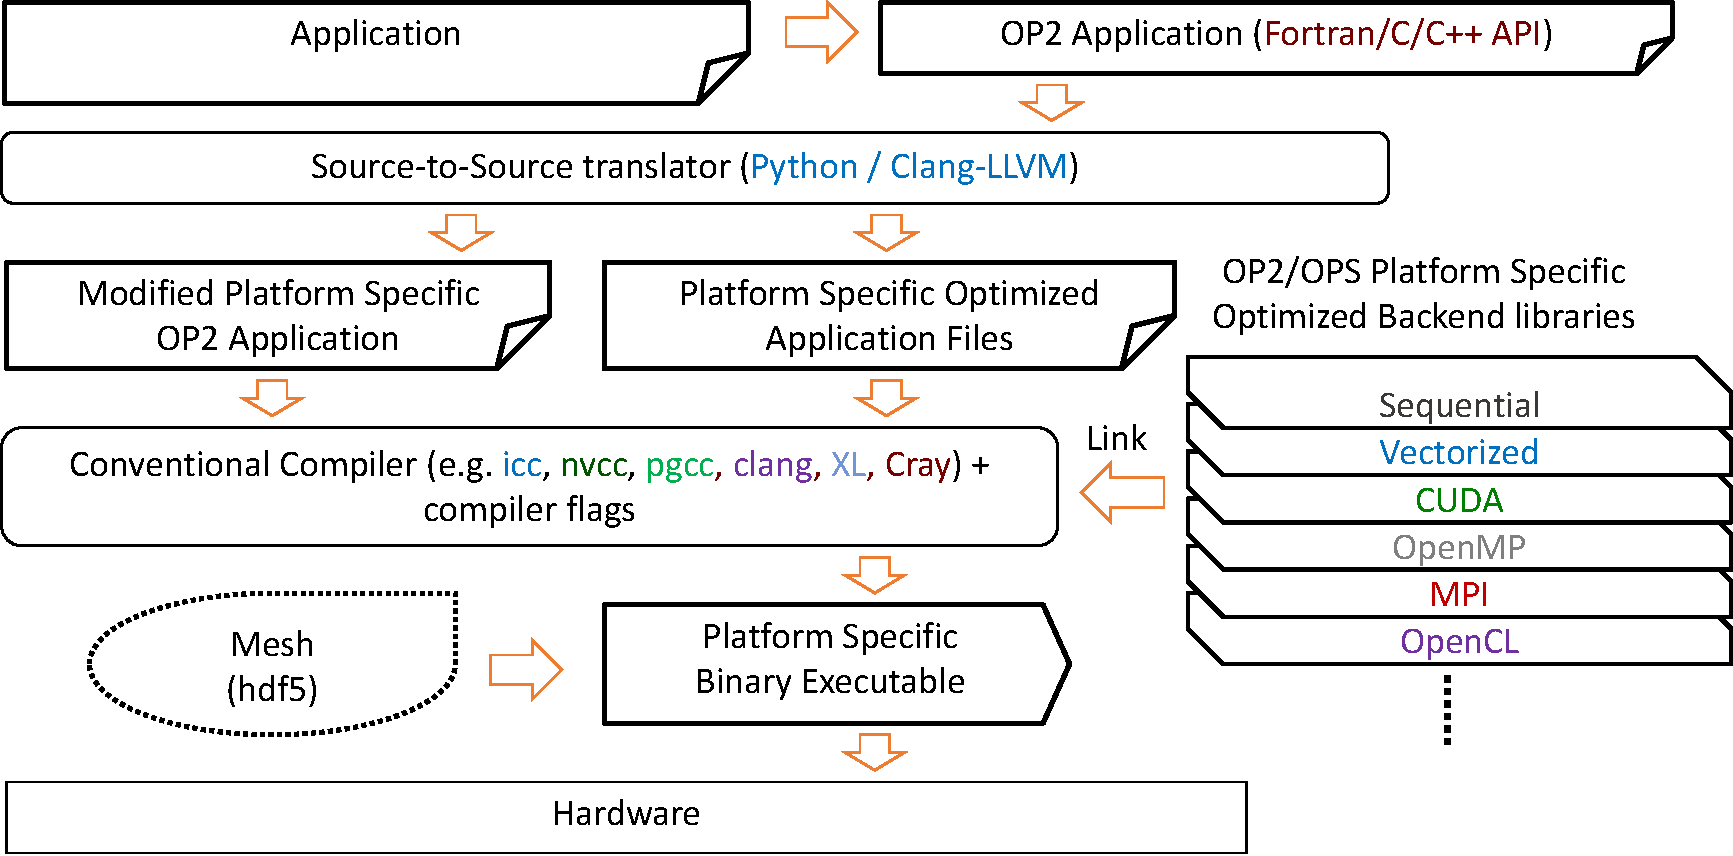
\includegraphics[width=9cm]{figures/flow}\vspace{-5pt}
\caption{Developing and Application with OP2}
\label{fig/op2flow}\vspace{-15pt}
\end{figure}



\vspace{-10pt}
\section{SYCL Parallelizations with OP2}\label{sec/op2sycl}
\vspace{-5pt}

\noindent The best performance we have observed with multi-threading on CPUs 
and SIMT on GPUs has been through the use of coloring and atomics, respectively. 
As such, for the SYCL implementation, we solely explore these strategies as 
appropriate to the target hardware. To ease the development of multiple 
parallelizations with a range of different optimizations, we make use of the 
OP2 DSL~\cite{op2repo,InPar2012}. 

OP2 allows to define the unstructured-mesh problem in four abstract components: 
(1) sets (e.g. nodes, edges, triangular faces, quadrilateral faces), (2) data on 
sets (e.g. node coordinates, edge weights, cell fluxes), (3) explicit 
connectivity (or mapping) between the sets and (4) operations over sets 
declared as kernels iterating over each element of the set, accessing indirectly 
via mappings. A simple example illustrating the OP2 API is presented 
in~\figurename{\ref{fig/op2api}}. The loop is over the set of edges, carrying 
out the computation per edge defined by the function \texttt{res}, accessing the 
data on edges, \texttt{p\_edge}, directly and  updating  the  data  held  on  
the  two  cells, \texttt{p\_cell}, adjacent to an edge, indirectly via the 
mapping \texttt{edge2cell}. The \texttt{op\_arg\_dat} provides details of how an 
\texttt{op\_dat}’s  data is accessed in the loop. Its first argument is the 
\texttt{op\_dat}, followed by its indirection index, \texttt{op\_map} used to 
access the data indirectly, arity of the data in the \texttt{op\_dat} and the 
type of the data. The final argument is the access mode of the data, read only, 
increment and others (such as read/write and write only, not shown here). The 
\texttt{op\_par\_loop} call contains  all  the  necessary information about the 
computational loop to perform the parallelization. It is clear that due to the 
abstraction, the parallelization depends only on a handful of parameters such as 
the existence of indirectly accessed data or reductions in the loop,  plus the 
data access modes that lends to optimizations. 

Parsing a code written in the above API, OP2's automatic code generator can 
produce a wide range of parallelizations following the development flow 
illustrated in~\figurename{\ref{fig/op2flow}}. When generating a platform 
specific parallel implementation of a loop specified by an 
\texttt{op\_par\_loop}, the code generator, essentially a source-to-source 
translator, makes use of a base template (or skeleton) that has been 
hand-crafted by the OP2 developers. Each of these skeletons make use of the 
best optimizations and platform specific configurations for the target hardware 
and programming models. For example, to produce the CUDA implementation, the 
OP2 code generator, simply modifies the appropriate CUDA skeleton with the 
declared parameters of the \texttt{op\_par\_loop} to produce the concrete 
implementation of the loop~\cite{OP2-Clang-Balogh2019}. Given the different 
parallelization strategies and optimizations that can be used even when using a 
single parallel programming model, different skeletons are maintained and reused 
together with configuration flags for further customizing what code they will 
generate. However, for a domain scientist developing an unstructured-mesh 
application, the process of generating a concrete parallel implementation will 
be automatic. In this work, we formulate the unstructured-mesh problem using 
OP2's domain specific abstraction and then extend its automatic code generation
tools to produce an optimized SYCL paralleization. Given the range of hardware 
and SYCL compilers available, multiple paralleization strategies were 
investigated to ascertain the best performance. On CPUs, we found that a 
hierarchical coloring strategy (with 1 work item per workgroup) to apply the 
indirect increments produced the best performance. On the NVIDIA GPUs 
benchmarked, the best performance with SYCL was achieved with atomics. However, 
a SYCL compiler exposing non-standard atomics is required to take advantage of 
the hardware support available on these many-core devices. 

\begin{figure}[t]
\begin{minted}[mathescape,
               linenos,
               numbersep=1pt,
               gobble=2,
               fontsize=\scriptsize,
               frame=lines, firstnumber=1,
               escapeinside=||,
               framesep=2mm]{c++}  
 op_par_loop(compute_flux_edge_kernel,
   "compute_flux_edge_kernel", op_edges,
   op_arg_dat(vars,0,en,5,"double",OP_READ),
   op_arg_dat(vars,1,en,5,"double",OP_READ),
   op_arg_dat(edwgts,-1,OP_ID,3,"double",OP_READ),
   op_arg_dat(fluxes,0,en,5,"double",OP_INC),
   op_arg_dat(fluxes,1,en,5,"double",OP_INC));
\end{minted}
\vspace{-20pt}\caption{MG-CFD's \texttt{compute\_flux\_edge\_kernel} loop}
\label{fig/comptfluxedge}\vspace{-15pt}
\end{figure}

\begin{figure}[!t]
\begin{minted}[mathescape,
               linenos,
               numbersep=1pt,
               gobble=2,
               fontsize=\scriptsize,
               frame=lines, firstnumber=1,
               escapeinside=||,
               framesep=2mm]{c++}
 /*Cast OP2 dats, maps and coloring plan as SYCL buffers*/
 arg0_buffer = ... ; // vars - indirectly accessed 
 arg3_buffer = ... ; // fluxes - indirectly accessed 
 map0_buffer = ... ; // en - mapping table
 arg2_buffer = ... ; // edwgts - directly accessed  

 col_reord_buffer = ... ; // coloring array

 for ( int col=0; col<Plan->ncolors; col++){//for each color
   int start = Plan->col_offsets[0][col];
   int end = Plan->col_offsets[0][col+1];
   int nblocks = (end - start - 1)/nthread + 1;
   
   // enqueue arguments and elemental kernel
   op2_queue->submit([&](cl::sycl::handler& cgh) {
     ind_arg0 = (*arg0_buffer).. // enqueue vars
     ind_arg1 = (*arg3_buffer).. // enqueue fluxes
     opDat0Map = (*map0_buffer).. //enqueue mapping en 
     arg2 = (*arg2_buffer).. // enqueue edwgts
     
     // enqueue coloring array
     col_reord = (*col_reord_buffer)..     
     // enqueue any global constants used in the kernel
     ...
     //elemental kernel function as lambda - enqueue it
     auto compute_flux_edge_kernel_gpu = [=]( 
        const double *var_a, const double *var_b,
        const double *edwgts,double *fluxes_a, 
        double *fluxes_b) 
        { .../*body of kernel*/... }; 
        
     // setup kernel work items
     auto kern = [=](cl::sycl::item<1> item) {  
       int tid = item.get_id(0);
       if (tid + start < end) {
         int n = col_reord[tid + start]; 
         int map0idx; int map1idx;

         // get the indirect index via mapping
         map0idx = opDat0Map[n+set_size*0]; 
         map1idx = opDat0Map[n+set_size*1];

         //user-supplied kernel call
         compute_flux_edge_kernel_gpu(
         &ind_arg0[map0idx*5], &ind_arg0[map1idx*5], 
         &arg2[n*3], 
         &ind_arg1[map0idx*5], &ind_arg1[map1idx*5]);
       }
     };   
     // execute kernel 
     cgh.parallel_for
     <class compute_flux_edge_kernel>
     (cl::sycl::range<1>(nthread * nblocks), kern);
   }); // end of enqueue arguments and elemental kernel
 }               
\end{minted}
\vspace{-20pt}\caption{Global coloring paralleization generated by OP2 for the
\texttt{compute\_flux\_edge\_kernel} loop in MG-CFD}
\label{fig/gblcoloring}\vspace{-20pt}
\end{figure}

\begin{figure}[t]\centering
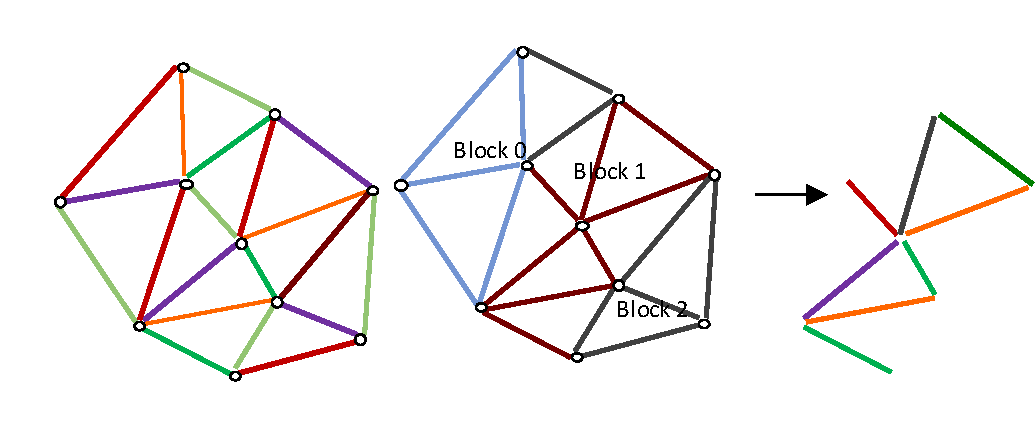
\includegraphics[width=9cm]{figures/coloring}\vspace{-15pt}
\vspace{-5pt}\caption{Coloring strategies in OP2 - global and hierarchical 
coloring}
\label{fig/coloring}\vspace{-15pt}
\end{figure}

\vspace{-10pt}
\subsection{Coloring}\label{subsec/coloring}
\noindent As noted before, coloring can be applied to resolve the data races in 
unstructured-mesh computations. This paralleization strategy can be generally
implemented on any shared memory multi-threaded system, including CPUs and 
GPUs without any restrictions due to hardware capabilities. Different 
variations of coloring have been implemented within OP2 as detailed in  
previous works~\cite{SULYOK201950}. Figure~\ref{fig/gblcoloring} details an 
excerpt of the SYCL code generated by OP2 for the most time-consuming 
parallel loop \texttt{compute\_flux\_edge \_kernel} in MG-CFD, our target 
unstructured-mesh CFD application. The OP2 API declaration of this loop  
is listed in Figure~\ref{fig/comptfluxedge}. The loop iterates over the mesh 
edges, \texttt{op\_edges}, indirectly reading DP floating-point data held on 
nodes in \texttt{vars}, using the edges to nodes, \texttt{en} mapping, 
directly reading DP floating-point data held on the edges in \texttt{edwgts} 
and indirectly incrementing data held on nodes in \texttt{fluxes}, again via 
the edges to nodes mapping.

There are two fundamental coloring schemes and execution strategies, which 
are illustrated in Figure \ref{fig/coloring}. The simpler one, called 
\emph{global coloring}, performs a single level of greedy coloring of set 
elements (in this case edges) based on a mapping (here edges to nodes). As the 
first drawing in Figure \ref{fig/coloring} shows, this gives us edge colors, 
where no two edges with the same color share a node. In terms of execution, 
edges with the same color can now be executed in parallel, with a 
synchronization between colors.

The second strategy, called \emph{hierarchical coloring}, performs two levels 
of coloring. First, the mesh is split into blocks of edges, the blocks 
themselves are colored, so that edges in different blocks of the same color do 
not share the same nodes. Second, edges within the block are colored. In terms 
of execution, blocks of the same color can be executed in parallel, and within 
blocks there is further parallelism, so edges of the same color can be executed 
in parallel. This hierarchical scheme maps to architectures with hierarchical 
parallelism, for example blocks map to OpenMP threads or thread blocks in CUDA, 
and intra-block parallelism maps to vector units or CUDA threads.

% Global Coloring 
The SYCL parallelization with global coloring starts by extracting the SYCL typed 
buffers from OP2's data structures (Figure~\ref{fig/gblcoloring}, lines 1-5). 
Each iteration over the loop's iteration set, in this case the mesh edges,  have 
been colored by OP2, held internally within a struct called \texttt{Plan}. This 
coloring information is stored in a SYCL integer buffer. A loop over number of 
colors, \texttt{ncolor}, starts execution over each edge with the same color in 
parallel (line 9). The list of edges belonging to the current color are held in 
the \texttt{col\_reord} array. The indices of the same color are held 
consecutively in this array. \texttt{start} and \texttt{end} are initialized to 
point to the start and end index for the current color respectively. The 
\texttt{Plan->col\_offsets} provides the required offset to jump to the correct 
index of the \texttt{col\_reord} array. 

Similar to the setup required for executing an OpenCL kernel, the 
arguments for the execution kernel, the kernel itself and any global constants 
referenced in the kernel are enqueued (lines 15-30). The kernel itself is 
specified as a lambda function (lines 25-30). Next, the SYCL kernel is setup 
such that \texttt{nblock} number of work-groups (i.e. blocks in CUDA parlance) 
each with \texttt{nthread} number of work-items, (i.e. threads in CUDA) are 
launched (lines 33-53). The indirections are resolved by using the edge index 
\texttt{n} to access the indices held in the mapping table \texttt{opDat0Map} 
(lines 40-41). The elemental kernel is called with these indices, together with 
the directly accessed data as arguments (lines 44-47).  

The advantage of global coloring is its simplicity - it can be easily expressed 
in any parallel programming environment. The main disadvantage with global 
coloring is the lack of data-reuse where multiple edges that write to the same 
mesh node have different color, and temporal locality is therefore poor. A 
further disadvantage is the low cache utilization where elements of the same 
color are not neighbors in the mesh, and therefore unlikely to be stored in 
consecutive memory locations. 

% Hierarchical coloring
The hierarchical coloring scheme maps well to GPU architectures, and in 
principle to CPU threads and vector units as well. However, the OpenMP-based 
implementations (hipSYCL, triSYCL) have a mismatch between the abstraction and 
the implementation, leading to extremely poor performance; they need to launch 
one thread per work item when using two-level parallelism (nd\_range). Intel's 
OneAPI compilers can optimise and map this better to hardware, yet despite 
achieving vectorization, performance was poor. To address these issues, we 
implemented a variation of the hierarchical execution scheme in SYCL where each 
work group consists of a single work item, which then iterates through the edges 
in that block sequentially. This proved to perform better on all CPU platforms 
with all compilers. This implementation now matches the execution scheme used by 
OP2's OpenMP execution scheme. However, it prevents vectorization by 
construction.

All coloring based executions add a one-time setup cost to the total runtime 
for creating the colored execution scheme. For production applications that 
iterate over many cycles, this setup cost becomes negligible or indeed could 
be pre-computed if the mesh is known before runtime. 

% Nevertheless, in this paper, we also present this overhead for MG-CFD executing 
% on our benchmark systems. 

% Why use set_size in the above code, when accessing via indirection?



% \subsection{Coloring}\label{subsec/coloring}
% Coloring can be applied to resolve the data races in unstructured-mesh 
% computations. This parallelization strategy can be generally implemented on 
% any shared memory multi-threaded system, including CPUs and GPUs without any 
% restrictions due to hardware capabilities. Different variations of coloring 
% has been implemented within OP2 as detailed in our previous 
% works~\cite{SULYOK201950}, where the two main variations being, global 
% coloring, and hierarchical coloring. Considering a loop over edges, that 
% updates indirectly the nodes connected to each edge, global coloring will 
% color the full iteration set (i.e. edges) such that no two edges with the same 
% color update the same node. The main disadvantage here, particularly on GPUs 
% is the lack of data-reuse where multiple iterations that write to the same 
% mesh node are scheduled for execution in different GPU kernel launches. A 
% further disadvantage is the low cache utilization where elements of the same 
% color are not neighbors in the mesh, and therefore unlikely to be stored in 
% consecutive memory locations. A hierarchical coloring in contrast, will 
% partition consecutive ``blocks'' of iterations into different colors such 
% that adjacent blocks are not assigned the same block-color. Within each 
% block, each edge is again colored such that no two edges with the same color 
% update the same node. This two level coloring has demonstrated improved cache 
% utilization, forming OP2's main coloring of choice for many-core hardware 
% without atomics support. 

% How op2 has used coloring in the past - varous coloring versions
% how we apply the same for a sycl parallelization (show with code segments if 
% appropriate)
% Coloring gives the best performance on modern CPUs (??)


\begin{figure}[!t]
\begin{minted}[mathescape,
               linenos,
               numbersep=1pt,
               gobble=2,
               fontsize=\scriptsize,
               frame=lines, firstnumber=1,
               escapeinside=||,
               framesep=0mm]{c++}  
 /*Cast OP2 dats, maps and coloring plan as SYCL buffers*/
 arg0_buffer = ... ; // vars - indirectly accessed 
 arg3_buffer = ... ; // fluxes - indirectly accessed 
 map0_buffer = ... ; // en - mapping table
 arg2_buffer = ... ; // edwgts - directly accessed  
 
 if (end-start>0) {
   int nblocks = (end-start-1)/nthread+1;        
   // enqueue arguments and elemental kernel
   op2_queue->submit([&](cl::sycl::handler& cgh) {
     
     ind_arg0 = (*arg0_buffer).. // enqueue vars
     ind_arg1 = (*arg3_buffer).. // enqueue fluxes
     opDat0Map = (*map0_buffer).. //enqueue mapping en 
     arg2 = (*arg2_buffer).. // enqueue edwgts
     // enqueue any global constants used in the kernel
     ...
     //elemental kernel function as lambda
     auto compute_flux_edge_kernel_gpu = [=](...)
     {  .../*body of kernel*/... };
      
     // setup kernel work items
     auto kern = [=](cl::sycl::nd_item<1> item) {             
       //local variables for holding indirect increments
       double arg3_l[5], arg4_l[5];
       for ( int d=0; d<5; d++ ){ arg3_l[d] = 0.0;}        
       for ( int d=0; d<5; d++ ){ arg4_l[d] = 0.0;}
       int tid = item.get_global_linear_id();
       if (tid + start < end) {
         int n = tid+start;
         int map0idx; int map1idx;
            
         // get the indirect index via mapping
         map0idx = opDat0Map[n + set_size * 0];
         map1idx = opDat0Map[n + set_size * 1];

         //elemental kernel call
         compute_flux_edge_kernel_gpu(
         &ind_arg0[map0idx*5], &ind_arg0[map1idx*5],
         &arg2[n*3], 
         arg3_l, arg4_l);
	    
	 //apply indirect increments using atomics
         {cl::sycl::atomic<double> a 
         {cl::sycl::global_ptr<double>
         {&ind_arg1[0+map0idx*5]}}; 
         a.fetch_add(arg3_l[0]);}
          ...
          ...
         {cl::sycl::atomic<double> a
         {cl::sycl::global_ptr<double>
         {&ind_arg1[4+map1idx*5]}}; 
         a.fetch_add(arg4_l[4]);}          
       }
     };
     // execute kernel 
     cgh.parallel_for
     <class compute_flux_edge_kernel>
     (cl::sycl::nd_range<1>(nthread*nblocks,nthread),kern);
   }); //end of enqueue arguments and elemental kernel
 }          
\end{minted}
\vspace{-15pt}\caption{Atomics-based paralelization generated by OP2 for 
\texttt{compute\_flux\_edge\_kernel} loop in MG-CFD}
\label{fig/atomics}\vspace{-20pt}
\end{figure}


\vspace{-10pt}
\subsection{Atomics}\label{subsec/atomics}
\vspace{-5pt}
\noindent In contrast to coloring, atomics based parallelizations enable the 
indirect updates (i.e. increments) applied one at a time using hardware atomic 
operations. The disadvantage is that not all hardware has fast DP 
implementations of atomics, and that the SYCL 1.2.1 standard does not include 
them, however hipSYCL has support for them on NVIDIA GPUs. 
Figure~\ref{fig/atomics} details an excerpt of the SYCL code generated by OP2 
for \texttt{compute\_flux\_edge\_kernel} loop using atomics targeting the 
hipSYCL compiler (which has support for DP atomics). The code, similar to the 
global coloring scheme for much of the setup code. The \texttt{start} and 
\texttt{end} now points to the full iteration range over the mesh edges. The key 
difference with atomics is the use of local arrays \texttt{arg3\_l} and 
\texttt{arg4\_l} to hold the indirect increments and apply them using atomics 
(lines 44-53). This results in an extra 10 floating point operations per edge. 
In contrast to coloring schemes, there is no setup cost for coloring plan 
construction when using atomics.  


% code segments of atomics written with SYCL - [can write this]

% The use of atomics, serializes the indirect updates by means of hardware 
% locks or atomic additions~\cite{SULYOK201950}. 

%  Atomics: where available atomics can be used to safely increment data. Note 
% that MG-CFD uses double precision, and those atomics are only supported on 
% NVIDIA hardware, and only exposed by the hipSYCL programming interface.

% using atomics in sycl - show with code segments if useful
% say that atomics provides the best performance on modern GPU hardware



\vspace{-10pt}
\section{Performance}\label{sec/perf}\vspace{-5pt}
\noindent In this section, we generate SYCL paralleizations with OP2 for MG-CFD 
\cite{Owenson2019}. MG-CFD is a 3D unstructured multigrid, finite-volume 
computational fluid dynamics (CFD) mini-app for inviscid-flow. Developed by 
extending the CFD solver in the Rodinia benchmark 
suite~\cite{RodiniaCFD2009,rodinia}, it implements a three-dimensional 
finite-volume discretization of the Euler equations for inviscid, compressible 
flow over an unstructured grid. It performs a sweep over edges to accumulate 
fluxes, implemented as a loop over all edges. Multi-grid support is implemented 
by augmenting the construction of the Euler solver presented 
in~\cite{RodiniaCFD2009} with crude operators to transfer the state of the 
simulation between the levels of the multi-grid. Initially written as a 
standalone CPU only implementation~\cite{Owenson2019}, MG-CFD has now been 
converted to use the OP2 API. It is available as open-source software 
at~\cite{mgcfd-op2}. This repository also contains the concrete parallel 
implementations generated through OP2 for SIMD, OpenMP, CUDA, OpenMP4.0, OpenACC 
and their combinations with MPI. The branch \texttt{feature/sycl} contains the 
generated SYCL versions of the application used in our performance 
investigation. 

% \begin{table*}[!t]\footnotesize
% \centering
% \caption{\small Benchmark systems specifications 
% \normalsize}\vspace{-8pt}
% \begin{tabular}{lllll} \hline
% System	    &	Kos		& Scyrus      & Isambard~\cite{GW4} & Node30	\\\hline
% Node	    &	Intel Xeon	& Intel Xeon  & Marvell ThunderX2  & AMD Ryzen\\
% Architecture&   E5-2660 v4 @ 2.00GHz (Broadwell) & Silver 4116 CPU @ 2.10GHz
%  & ARMv8.1 @ 2.1GHz & Ryzen 7 2700 @ 3.20 Ghz  \\
% 	    & + 1 $\times$ Nvidia Tesla V100 GPU (PCIe) & (Skylake)  & &  (Zen+) \\	
% 	    & + 3 $\times$ Nvidia Tesla P100 GPUs (PCIe) &	&  & + 1 x AMD Radeon VII \\
% 	    &&&&GPU
% 	    \\\hline
% Procs $\times$ cores &	2$\times$14 (2 SMT/core)   &	2$\times$12 (2 SMT/core)
% &  2$\times$32 (4 SMT/core) & 1x8 (2 SMT/core)	   \\\hline
% CPU Vector Length	 & CPU not used	&  512 bits  & 128 bits & CPU not used\\
% (Instructions) & 	&  (AVX-512)       &  (NEON) \\\hline
% Cache Hierarchy & 64 KB shared L1/SM (P100) &  64KB L1/core,  &  32KB L1/core & 16 KB shared L1/CU  \\
% 		&  	128 KB shared L1/SM (V100)		 &  1MB L2/core, & 256KB L2/core & 4MB shared L2\\
% 	        &   4MB shared L2 (P100)                     &  16.5MB L3/socket,& 32MB L3/socket \\
% 	        & 6MB shared L2 (V100)
% \\\hline
% CPU Main Memory    & 132 GB &  96 GB       & 256 GB  & 32 GB  \\
% GPU Global Memory  &  16GB (P100) and 16GB (V100) &    & & 16 GB \\\hline
% O/S	    & Debian 4.9.51 	&  Debian 4.9.82       & Cray PE with CCE 8.7.9	& CentOS 7.6.1810
%     \\\hline
% TDP per CPU or GPU  & 105 W (1$\times$ Broadwell)    & 85W (1 x Skylake) & \texttildelow180W (1 
% x ThunderX2)  & 65 W (1 x Zen+)\\
% & 250 W (1$\times$ V100 or P100) &       &  & 295 W (1$\times$ Radeon VII) \\\hline   
    
% \end{tabular}\label{tab/systems}\vspace{0pt}
% \end{table*}\normalsize


\begin{table*}[!t]\footnotesize
\centering
\caption{\small Benchmark systems specifications: GPUs
\normalsize}\vspace{-8pt}
\begin{tabular}{lllll} \hline
GPU	    &	NVIDIA V100		& NVIDIA A100      & AMD Radeon VII	& Intel Iris XE MAX	\\\hline
Form factor & PCI-e 3.0 & SXM4 & PCI-e 3.0 &PCI-e 4.0 \\\hline
Cores & 5120 & 6912 & 3840 & 768 \\\hline
Clock (MHz) & 1245-1380 & 1410 & 1400-1750 & 300-1650 \\\hline
TFLOPS/s compute & 7 & 9.7 & 3.46 & 2.53 (single) \\\hline
Bandwidth (GB/s) & 900 & 1600 & 1024 & 68 \\\hline
Memory size (GB) & 16 & 40 & 16 & 4 \\\hline
TDP (W) & 250 & 400 & 300 & 25 \\\hline
\end{tabular}\label{tab/systems1}\vspace{-15pt}
\end{table*}\normalsize


\begin{table*}[!t]\footnotesize
\centering
\caption{\small Benchmark systems specifications: CPUs
\normalsize}\vspace{-8pt}
\begin{tabular}{llll} \hline
System	    &	AWS c5d.24xlarge		& AWS c5a.24xlarge      & AWS c6g.16xlarge		\\\hline
Node	    &	Intel Xeon	& AMD Epyc (\textbf{Rome}) & AWS \textbf{Graviton2}  \\
Architecture&   Platinum 8275CL @ 3.00GHz & 7R32 @ 3.20GHz 
 &ARM v8.2 @ 2.5GHz   \\
 & (\textbf{Cascade Lake}) &&
 \\\hline
Procs $\times$ cores &	2$\times$24 (2 SMT/core)   &	1$\times$48 (2 SMT/core)
&  1$\times$64 (1 thread/core)	   \\\hline
CPU Vector Length	 &  512 bits  & 256 bits & 128 bits \\
(Instructions) & (AVX-512)	&  (AVX-2)       &  (NEON) \\\hline
Cache Hierarchy &  64KB L1/core,  &  64KB L1/core & 64KB L1/core  \\
		 &  1MB L2/core, & 512KB L2/core & 1MB L2/core\\
	        &  35.75MB L3/socket& 256MB L3/socket & 32MB L3/socket
\\\hline
CPU Main Memory    & 192 GB &  192 GB       & 128 GB  \\\hline
O/S	    & Ubuntu 20.04 	&  Ubuntu 20.04       & Ubuntu 20.04\\\hline
TDP per CPU & \texttildelow240 W   & \texttildelow220W & \texttildelow100W  \\\hline   
    
\end{tabular}\label{tab/systems2}\vspace{0pt}
\end{table*}\normalsize



\begin{table*}[!t]\footnotesize
\centering
\caption{\small Compilers and Compiler Flags
\normalsize}\vspace{-8pt}
\begin{tabular}{lllll} \hline
Compiler	    &	Version 	& Compiler Flags\\\hline
Intel OneAPI Compilers     &	Beta 9 	& \texttt{-O3 -xHOST  -inline-forceinline } \\
\texttt{icc, icpc, dpcpp}  & &\texttt{ -restrict -qopenmp|-fsycl}  \\\hline
\texttt{nvcc}  	    &   CUDA 10.2  	&  \texttt{-O3 -restrict}\\
&&V100 : \texttt{-gencode 
arch=compute\_70,code=sm\_70} \\
&& A100 : \texttt{-gencode arch=compute\_80,code=sm\_80} \\\hline
HipSYCL Compiler & Based on Clang 9 & \texttt{-O3}\\
&& All CPUs: \texttt{--hipsycl-platform=cpu} \\
\texttt{syclcc-clang}&&V100 : \texttt{--hipsycl-gpu-arch=sm\_70} \\
&& A100 : \texttt{--hipsycl-gpu-arch=sm\_80} \\
&& Radeon VII : \texttt{--hipsycl-gpu-arch=gfx906} \\\hline
GNU 	    &   9.3 &  AMD Rome, AWS Graviton2 \texttt{-Ofast -fopenmp}  \\ 
\texttt{gcc,g++}     &  &   \texttt{ } \\\hline
\end{tabular}\label{tab/compilers}\vspace{-15pt}
\end{table*}\normalsize
% Table with specifications and text with details 






% The first system, Kos is a single node system consisting of 
% two Intel Xeon Broadwell processors together with 
% multiple Nvidia GPUs: 1$\times$ Tesla V100 and 3$\times$ Tesla P100s, 
% each with 16~GB of global memory~\cite{P100TDP, V100TDP}. 
% We only make use of the V100 and one P100 GPU from this system in this paper. 
% %Both the GPUs have 16~GB of global memory~\cite{P100TDP, V100TDP}. 
% The second system, Scyrus, consists of two Intel 
%Skylake~\cite{XeonSilver4116TDP} processors, each consisting of 12 cores. 
%Each core is configured to have 2 hyper-threads. The 
%processor consists of 768~KBs of L1 instruction and data caches per core, 1MB 
%of L2 caches per core and 16.5 MBs of L3 cache per socket. The Skylake 
% %architecture also has a SIMD vector length of 512 bits allowing to execute Intel 
% %AVX-512 vector instructions. 
% each contains 12-cores with hyper-threading enabled (2-wide SMT), 
% and provides 512-bit vectorization using AVX-512 instructions. 
% The third system is a single node from the Cray 
% XC50 ARM system ``Isambard'' ~\cite{GW4}, located at one of UK's Tier-2 national HPC 
% sites. The node consists of two Marvell ThunderX2 ARMv8.1 processors, each with 
% %32 cores each. 
% %Each core has 4 threads (SMTs) and consists of a 32KB of L1 
% %instruction and data cache per core, 256KB of L2 cache per core and 32MB of L3 
% %cache per processor. 
% 32 cores and 4-wide SMT, and 128-bit vectorization using NEON instructions. 
% The final system is a node with an AMD Ryzen 7 2700 processor, and an AMD Radeon VII GPU 
% with 6~GB of global memory \cite{RadeonVIIspec}. 
% Similar to Kos, we are only interested in the Radeon GPU and are not testing the Ryzen CPU. 
% The Radeon has 16~GB of global memory \cite{RadeonVIIspec}.
Our aim is to compare the performance of the SYCL implementations to that of 
other parallel versions for MG-CFD and explore how similar execution strategies 
can be expressed using SYCL. For benchmarking we make use of a number of 
systems based on currently prevalent and emerging processor architectures. A 
summary of the key specifications of these systems are detailed 
in~\tablename{~\ref{tab/systems1}} and ~\tablename{~\ref{tab/systems2}}. \\
\indent The NVIDIA V100 and AMD Radeon VII GPUs we accessed directly in our 
systems. The A100 GPUs used were in AWS \texttt{p4d.24xlarge} instances, and the 
Iris XE MAX (Based on XE LP architecture) GPUs were accessed through Intel's 
DevCloud. To benchmark CPUs, we have evaluated three high-end machines available 
through Amazon Web Services (AWS). The \texttt{c5d.24xlarge} instance has a 
dual-socket Intel Xeon Platinum CPU, from the Cascade Lake generation, each with 
24 cores and 2 threads per core. The \texttt{c5a.24xlarge} has a single socket 
AMD Epyc Rome generation CPU with 48 physical cores and 2 threads per core. The 
\texttt{c6g.16xlarge} has a single socket AWS Graviton2 ARM CPU with 64 cores. 
While all of these were virtual machines, these contain some of the latest 
hardware architectures available, and achieve the same fraction of peak 
performance as our internal, less powerful, Intel-based bare-metal systems.
%, and as we show performance is comparable or better than the 
% bare-metal machines listed in~\tablename{~\ref{tab/systems}}.
% Runtime performance and Speedups comparison (add notes of compilers used for 
% each)

\begin{figure*}[t]
\centering
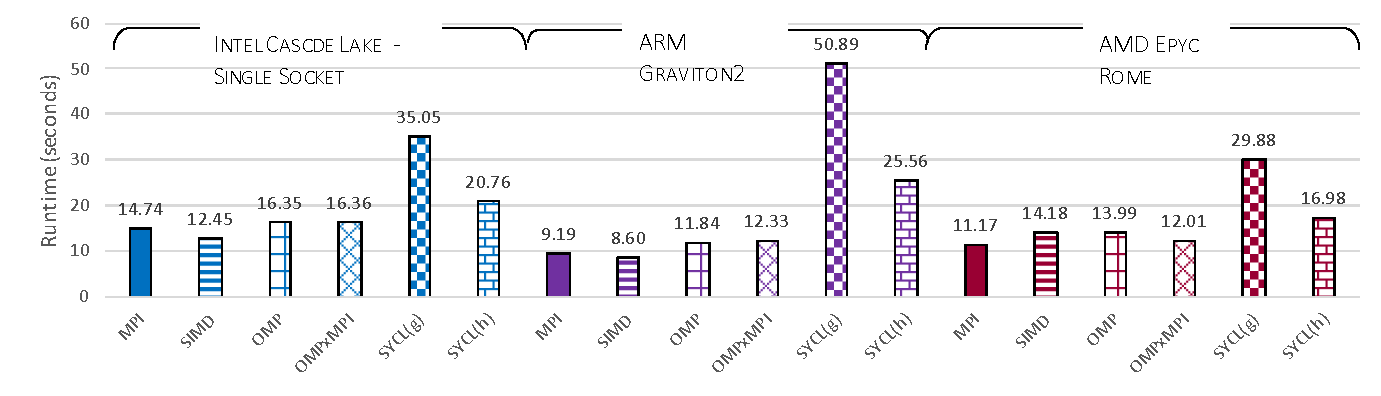
\includegraphics[width=12.5cm]{figures/SingleNode1SKTPerf}\vspace{-0pt}
\vspace{-22pt}\caption{MG-CFD, Runtime (seconds) on single socket CPUs - 8M 
edges, 25 MG Cycles }
\label{graph/perf}\vspace{-5pt}
\end{figure*}
% \begin{figure*}[t]
% \centering
% 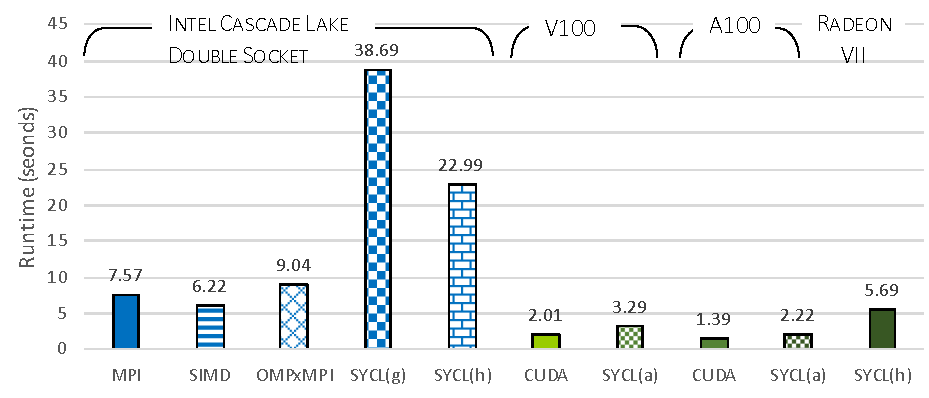
\includegraphics[width=18.5cm]{figures/SingleNode2SKTPerf}\vspace{-0pt}
% \caption{MG-CFD, Normalized Performance-per-Watt - 8M edges, 25 MG 
% Cycles (higher is better)}
% \label{graph/powerperf}\vspace{-10pt}
% \end{figure*}

\begin{figure*}[t]
\centering
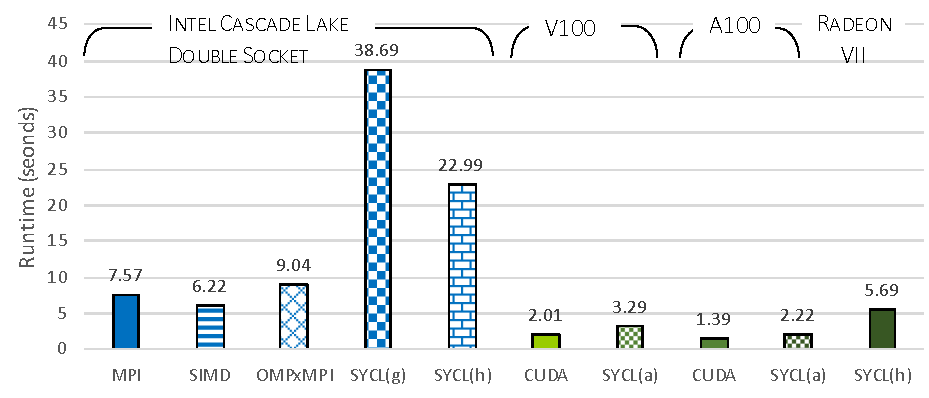
\includegraphics[width=10cm]{figures/SingleNode2SKTPerf}
\vspace{-10pt}\caption{MG-CFD, Runtime (seconds) on a dual socket CPUs and GPUs 
- 8M edges, 25 MG Cycles }
\label{graph/perf2}\vspace{-15pt}
\end{figure*}

Figures~\ref{graph/perf} and ~\ref{graph/perf2} presents the runtime of the 
main time marching loops of MG-CFD on the above systems solving a NASA Rotor 37 
\cite{rotor37} benchmark mesh consisting of 8 million edges on the finest level. 
The time to solution of 25 multi-grid cycles are reported here. The time 
for initial I/O (mesh loading and partitioning) are not included, given that 
these are a one-off setup cost and depends on other libraries such as HDF5, 
ParMetis/PTScotch etc., whose performance is not the subject of this paper. The 
figure presents the runtime of the application without any coloring plan time 
construction overheads, which was discussed in Section~\ref{subsec/coloring}. 
Given these setup costs are one-off or indeed can be computed a priori if the 
mesh is known before runtime, we believe the figure provides a fairer 
comparison between the actual performance of each architecture and 
parallelization model. 
%Nevertheless, these overheads have been included in 
%% TODO: broken reference:
%Figure~\ref{table/plantimes} 
%for completeness of the results. 
Compilers and 
compiler flags used for each version of the parallelizations are detailed 
in~\tablename{ \ref{tab/compilers}}. 

Reference performance numbers were collected using existing parallelizations in 
OP2; plain MPI which does not auto-vectorize, an MPI+SIMD version which uses 
explicit gathers and scatters to enable auto-vectorization, OpenMP that does not 
auto-vectorize, hybrid MPI+OpenMP, and for NVIDIA GPUs, CUDA using atomics.

On the Intel Cascade Lake CPU, we used the OneAPI compilers to compile SYCL. The 
global colouring variant \emph{(g)} uses a flat parallel for loop, however due 
to poor memory access patterns it performs the worst. To improve memory 
locality, we utilize the hierarchical execution scheme \emph{(h)} - mapping 
blocks to threads as done in case of OpenMP, and optionally elements in blocks 
to vector lanes. The performance reported in Figure \ref{graph/perf} (SYCL (h)) 
uses the same number of blocks as the OpenMP version and only uses a single work 
item per workgroup, which mirrors the behavior of our OpenMP execution scheme, 
and is $26\%$ slower. This was confirmed by inspecting the generated assembly. 
We also evaluated using 8 work items (AVX512 with FP64) and utilized Intel's 
subgroup extension to perform safe colored updates, however performance did not 
improve. An examination of the generated assembly for the most expensive loop 
provides two key insights : (1) computations did vectorize, closely matching our 
SIMD variant, although no fused multiply-add instructions were generated, (2) 
the number of memory movement operations were significantly larger (approx. 
$2\times$).

On the ARM Graviton2 and AMD Epyc CPUs, we used the hipSYCL implementation of 
the standard, which uses OpenMP underneath. For flat parallel loops hipSYCL will 
map computations to a flat OpenMP parallel loop, however, when using 
hierarchical parallelism it will launch one thread per work item to guarantee 
that barriers can be handled correctly. The global coloring execution scheme 
clearly performs poorly, due to the lack of memory locality. For the 
hierarchical execution scheme, we used a single work item per workgroup, 
mirroring the OpenMP execution scheme. On the Graviton2 SYCL performance is 
$2.16\times$ worse than plain OpenMP - largely due to the relative immaturity of 
ARM support in Clang (used by hipSYCL) versus GNU g++ (used with flat OpenMP). 
On the AMD Epyc however, SYCL performs only $21\%$ slower compared to plain 
OpenMP.

For the comparison with GPUs, we also ran on both sockets of the Intel Cascade 
Lake CPU, and observed over $95\%$ scaling efficiency for pure MPI and MPI+SIMD, 
though only $80\%$ for MPI+OpenMP. SYCL however did not improve when running 
over both sockets due to NUMA issues - OP2 does not yet have an MPI+SYCL 
backend. For both NVIDIA and AMD GPUs, we made use of the automatic 
Array-of-Structs to Struct-of-Arrays data layout conversion feature of OP2. On 
NVIDIA GPUs, we used the atomics versions and compiled with hipSYCL - showing a 
$60-64\%$ slowdown compared to the atomics version of CUDA. The differences are 
likely due to the immaturity of the hipSYCL compiler, resulting in higher 
register pressure and worse occupancy.The AMD Radeon VII GPU does not have 
hardware support for double precision atomics, and therefore we utilized the 
hierarchical coloring execution scheme with 128 work items per workgroup. OP2 
does not have support for either HIP or OpenCL, therefore we could not compare 
this to a reference implementation.

\vspace{-10pt}
\subsection{Intel Iris XE MAX}
\vspace{-5pt}

To further explore OneAPI, we have evaluated the recently released Intel 
datacenter GPU built on the XE LP (low-power) platform. As the specifications in 
Table \ref{tab/systems1} show this is a GPU in an entirely different class to 
the others tested. It has a $10-16\times$ lower TDP, and a similarly lower 
maximum bandwidth (53 GB/s measured bandwidth), yet a relatively high maximum 
computational throughput - though it has to be noted that the card does not 
support double precision. This makes the platform have the highest FLOPS to 
bandwidth ratio among all the tested hardware. 

We prepared a single precision version of MG-CFD to evaluate performance - 
without considering the implications on accuracy and convergence at the moment. 
These GPUs also do not support single precision atomics, therefore we evaluated 
the various colored execution schemes. Intel's GPUs also support the subgroups 
extension of SYCL, and indeed are vital for good performance. We found the best 
performing combination to use the hierarchical coloring execution scheme with 16 
work items per workgroup, and 16 work items per subgroup (i.e. one subgroup per 
workgroup), and relied on subgroup barriers to perform the colored updates. The 
automatic AoS to SoA data layout conversion did not improve performance on this 
GPU. The best runtime was 22.37 seconds - to put this result in context, we 
compared performance to a single-socket Platinum 8256 CPU (4 cores, 51 GB/s 
STREAM bandwidth), which ran MPI+SIMD in 21.62 seconds and pure OpenMP in 42.37.

% The best SYCL performance on CPUs were obtained with the hipSYCL compiler 
% ~\cite{hipsycl} on the AMD Epyc processor node. hipSYCL, when targeting CPUs, 
% maps the SYCL execution model to an OpenMP execution model to run codes in 
% parallel. Second best performance is achieved on the Intel Xeon Platinum CPU, 
% utilizing the OneAPI toolkit \cite{intel-sycl}. This compiler is based on the 
% LLVM-Clang compiler, but extended by Intel to support compiling SYCL to 
% SPIR-V, which is then further compiled by Intel's OpenCL drivers. For CPUs, we 
% evaluate performance with global coloring, marked with \texttt{(g)} and 
% hierarchical coloring, marked with \texttt{(h)}. The latter uses a single work 
% item per work group (mapped to a single OpenMP thread with hipSYCL) - and 
% performs consistently better than the global coloring variant.
%coloring, as discussed in~\cite{SULYOK201950}, has been used to resolve race 
%conditions when parallelizing the application. Atomics are not available on these 
%CPUs (and generally no atomics are implemented on any modern CPU). We did 
%experiment with Codeplay's compute++~\cite{compute++} and the 
%hipSYCL~\cite{hipsycl} compilers but we found that the Intel SYCL compiler was 
%consistently more 
%stable. 
%% What do you mean by "stable"? Did compiler/mg-cfd crash sometimes? 

% Because the Intel SYCL compiler does not support non-Intel CPU platforms, 
% hipSYCL was chosen to generate code for execution on ARM and AMD CPUs, as other 
% compatible compilers such as compute++ were unreliable (failed to compile, run 
% or gave incorrect results) in our tests. hipSYCL was also the only compiler 
% exposing atomics 
% that can be used on Nvidia GPUs. Since hipSYCL uses the HIP backend, it also 
% allows us to run the code on the Radeon VII due to hipSYCL's support of ROCm. It 
% is worth noting that while atomics can be enabled on the Nvidia GPUs, they are 
% not available on the Radeon GPU being tested.



% As detailed in Figure \ref{graph/perf} and \ref{graph/perf2}, the application 
% compiled with the Intel 
% SYCL compiler was 40\% slower than the 48 rank MPI version, and 27\% slower than 
% the pure OpenMP case. Compared to the MPI+SIMD versions on a 
% single CPU socket, the SYCL version was about 66\% 
% slower. We believe this presents an accurate reflection of the 
% current performance on recent Intel CPUs. It is very likely that performance 
% will improve over time as both the Intel SYCL compiler and the standard itself 
% matures further.

% For the ARM system, SYCL performance is 23\% worse than the Intel SYCL result, 
% which can be put down to the different approaches of Intel's SYCL compiler and 
% hipSYCL. Since hipSYCL is a translation layer, the performance gap to Intel's 
% solution, which is a low level and vendor specific implementation, is not 
% surprising. This can be further seen when compared to the ARM MPI result, which 
% is significantly better than the SYCL result - indeed, it is the fastest 
% single socket CPU result, owing to the highest available bandwidth. 

% The Intel Cascade Lake processor gains 18\% performance when explicitly 
% utilizing 
% the 512-bit SIMD vector units.  The ARM processor node also gains 8\% 
% performance with the SIMD implementation, despite only having 128 bit vectors. 
% In contract, on the AMD EPYC, performance degrades, despite having 256 bit 
% vectors. We used GCC to compile for both ARM and AMD, but of course the two use 
% completely different instruction sets. %TODO: not much explanation here...

% Considering the NVIDIA GPU performance we see that the SYCL versions, using 
% atomics, are only about 20\% and 29\% slower than the CUDA versions on the P100 
% and V100 GPUs respectively, as seen in Figure~\ref{graph/perf}. On the Radeon 
% % VII, we do not have a different implementation to compare against - double 
% precision atomics are not supported, therefore we used coloring. These 
% SYCL versions were compiled with the hipSYCL compiler, which uses HIP~\cite{hip} 
% to convert SYCL code into CUDA and ROCm equivalents (as opposed to OpenCL). 
% As the results show, while the runtimes are slower than using atomics, HIP's 
% easy porting of code to different devices makes this is a worthwhile trade-off. 
% For example, there is no HIP code generation yet supported by OP2, but the 
% SYCL extensions allow us to run on the AMD Radeon hardware.

% Comparing the overall runtime performance on both CPUs and GPUs, the CUDA 
% version on the P100 and V100 GPUs is 1.5$\times$ and 3.1$\times$ respectively 
% faster than the best performing parallelization (MPI with SIMD vectorization) on 
% the dual-socket Intel node. 
%The Radeon VII SYCL version was the fastest out of all 
%systems tested, being 6.0 $\times$ faster than the best CPU run given 
%by MPI+SIMD on the Skylake. One important observation to note here is that  
%the plan time for the Radeon GPU was high, as seen in Figure 
%\ref{table/plantimes}. This may be due to the small L1 cache sizes of the Vega20 
%architecture causing bottlenecks in the coloring stage. However, with a larger 
%number of multi-grid cycles, this overhead would be amortized.

% \begin{table*}\footnotesize
% \begin{center}
% \begin{tabular}{|l|r|r|r|} \hline
% System and Run & Runtime (s) & Plan time (s) & Runtime w/o plan time (s) \\ 
% [0.5ex] \hline\hline
% %  Skylake (48MPI) & 14.22 & 0.00 & 14.22\\\hline
% %  Skylake (48MPI+SIMD) & 12.27 & 0.00 & 12.27\\\hline
% %  Skylake (24MPI) & 17.20 & 0.00 & 17.20\\\hline
% %  Skylake (24MPI+SIMD) & 14.44 & 0.00 & 14.44\\\hline
%  Skylake (2OMP\ \times\ 24MPI) & 22.44 & 1.64 & 20.80\\\hline
%  Skylake (SYCL - 48SMT, Global coloring) & - & - & 15.58\\\hline
% %  ThunderX2 (64MPI/Clang) & 16.89 & 0.00 & 16.89\\\hline
% %  ThunderX2 (64MPI+SIMD/Clang) & 26.26 & 0.00 & 26.26\\\hline
%  ThunderX2 (4OMPx64MPI) & 20.40 & 0.87 & 19.53\\\hline
%  ThunderX2 (64 SMT, Global coloring, hipSYCL) & 71.75 & 33.19 & 38.56\\\hline
% %  P100 (CUDA, Atomics) & 5.31 & 0.00 & 5.31\\\hline
% %  P100 (Atomics/hipSYCL) & 6.38 & 0.00 & 6.38\\\hline
% %  V100 (CUDA, Atomics) & 3.20 & 0.00 & 3.20\\\hline
% %  V100 (Atomics/hipSYCL) & 4.15 & 0.00 & 4.15\\\hline
%  AMD Radeon VII (Global coloring, hipSYCL) & 18.77 & 16.74 & 2.03\\\hline
% \end{tabular}
% \end{center}
% \caption{Runtimes and Plan times for parallelizations using coloring}
% \label{table/plantimes}
% \vspace{-13pt}
% \end{table*}\normalsize

% When considering power consumption, the Skylake system is the most power 
% efficient, with a TDP of only 85W per socket. The NVIDIA GPUs each have a high 
% TDP of 250W, but since their performance is strong, they have superior 
% performance-per-watt, as seen in Figure \ref{graph/powerperf}. The Radeon VII 
% has exceptional performance-per-watt, which is due to a combination of high 
% performance and low power consumption of the host system, consisting of a single 
% Ryzen 7 2700 processor. The high power draw of the ThunderX2 CPUs in the 
% Isambard system, combined with weak performance, means it has a poor 
% performance-per-watt value. 

% It can also be seen that since SYCL performance is close to the reference 
% builds, the predominant factor in performance-per-watt in this case is the 
% device itself, and not the API. Moving from a single socket Xeon Skylake to dual 
% socket brings little performance increase, but will double the CPU power usage. 
% Running 2S SIMD is only 0.55x as efficient as running 1S SIMD; this is most 
% likely due to the latency of scatter-gather when using 2 sockets limiting 
% performance.

% It should be noted that our comparisons are done with approximate power 
% consumption numbers, and thus performance-per-watt metrics are only an estimate. 
% Variability in power draw from the chipset, memory, storage, or other 
% components, which can consume more power than the CPU or GPU itself 
% \cite{Marta2016}, may result in inaccuracies in the calculation. In addition, 
% TDP specifications may be exceeded depending on the workload; for example using 
% SIMD consumes significantly more power than ordinary compute 
% \cite{gottschlag2018mechanism}. However, we believe our results are an accurate 
% representation of the performance and efficiency of these systems.

% Estimate Power draw (for comparison) -use estimated TDPs


% \begin{figure*}
% \vspace{1cm}
% \begin{subfigure}[t]{\textwidth}
% \centering
% \begin{tikzpicture}
% \tikzstyle{every node}=[font=\small]
% \begin{axis}
%     [
%         legend cell align={left},
%         area legend,
%         width=12cm,
%         height=7cm,
%         enlarge x limits=0.1,
%         ylabel={Performance-per-watt},
%         bar width=0.4cm,
%         font=\rmfamily\scriptsize,
%         xtick=data,
%         ymin=0,
%         ymax=1.8,
%         nodes near coords,
%         nodes near coords style={/pgf/number format/.cd,fixed 
% zerofill,precision=2},
%        xtick={Intel SIMD 1S, Intel SIMD 2S, Intel SYCL, Isambard MPI 2S, P100 
% CUDA, P100 SYCL, V100 CUDA, V100 SYCL},
%        x tick label style={text width=1cm,align=center},
%        symbolic x coords={Intel SIMD 1S, Intel SIMD 2S, Intel SYCL, Isambard MPI 
% 2S, P100 CUDA, P100 SYCL, V100 CUDA, V100 SYCL},
%    ] \addplot [ybar, fill=blue!30!white] coordinates {
%        (Intel SIMD 1S, 1.00) (Intel SIMD 2S, 0.59) (Intel SYCL, 0.46) (Isambard 
% MPI 2S, 0.40) (P100 CUDA, 0.92) (P100 SYCL, 0.77) (V100 CUDA, 1.53) (V100 SYCL, 
% 1.09)
%     };
% \end{axis}
% \end{tikzpicture}
% \end{subfigure}
% \caption{Normalized Performance-per-watt (fastest run for each configuration)}
% \label{graph/perfperwatt}
% \end{figure*}

% \begin{figure}[t]\hspace{-0pt}\footnotesize 
% 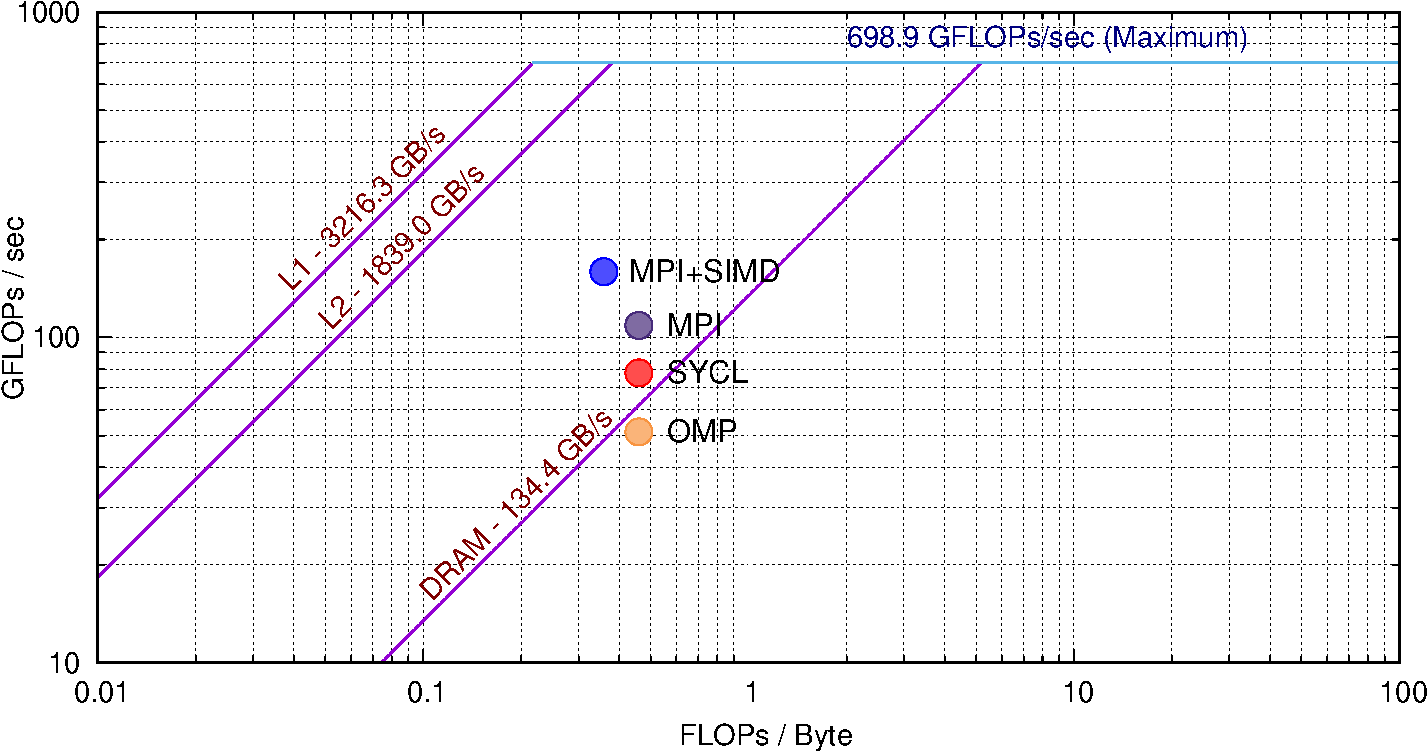
\includegraphics[width=9cm]{Rooflines/Roofline_SkyLake} \vspace{-14pt}
% \caption{Roofline plot of the Skylake system, showing 48 MPI ranks + SIMD, 48 
% MPI ranks, 2 socket SYCL, and 2 OpenMP threads + 24 MPI ranks}
% \label{graph/perf/skylake/roofline}\vspace{-10pt}
% \end{figure}\normalsize

% \begin{figure}[t]\hspace{-0pt}\footnotesize
% 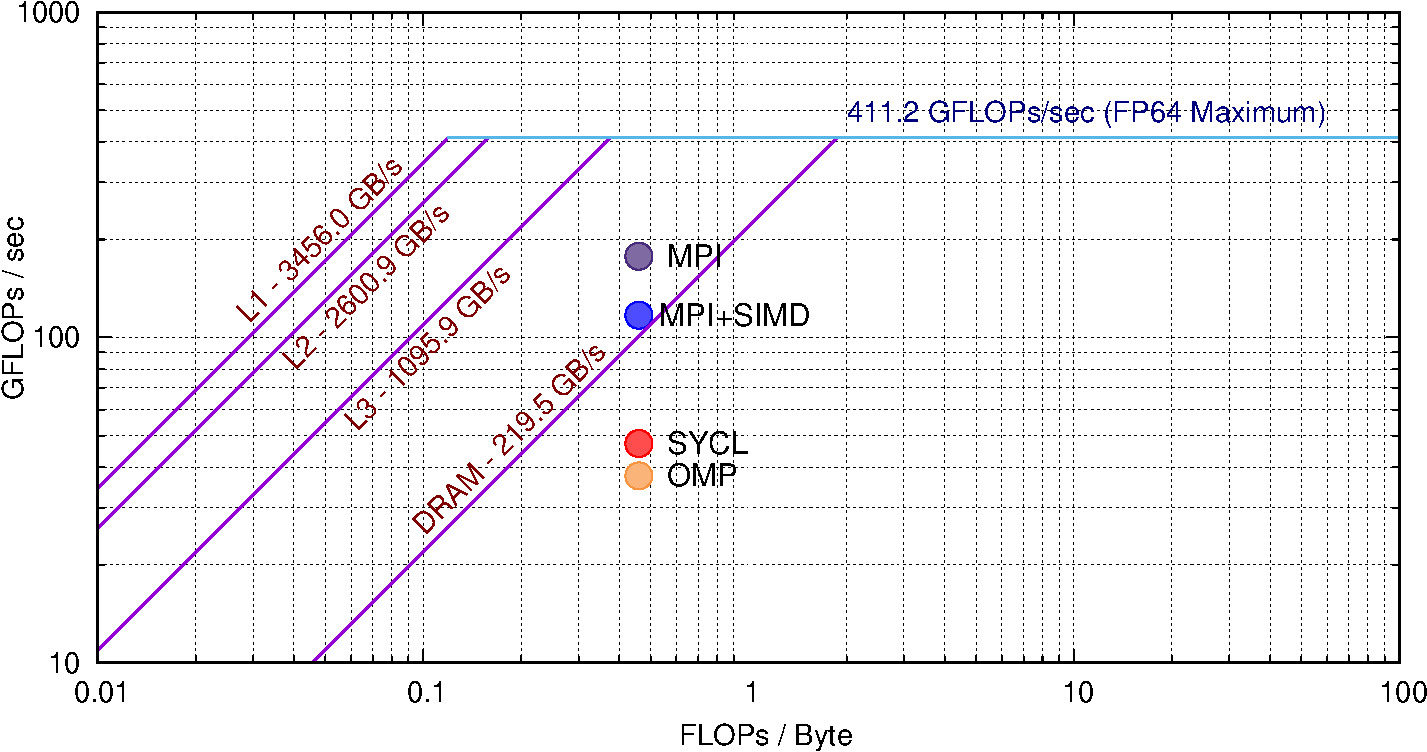
\includegraphics[width=9cm]{Rooflines/Roofline_Isambard} \vspace{-14pt}
% \caption{Roofline plot of the Isambard system, showing 64 MPI ranks, 64 MPI 
% ranks + SIMD, single socket SYCL, and 4 OpenMP threads + 64 MPI ranks}
% \label{graph/perf/isambard/roofline}\vspace{-10pt}
% \end{figure}\normalsize


% \begin{figure*}[t]\centering   \footnotesize 
% \begin{subfigure}{.32\textwidth}\centering
% 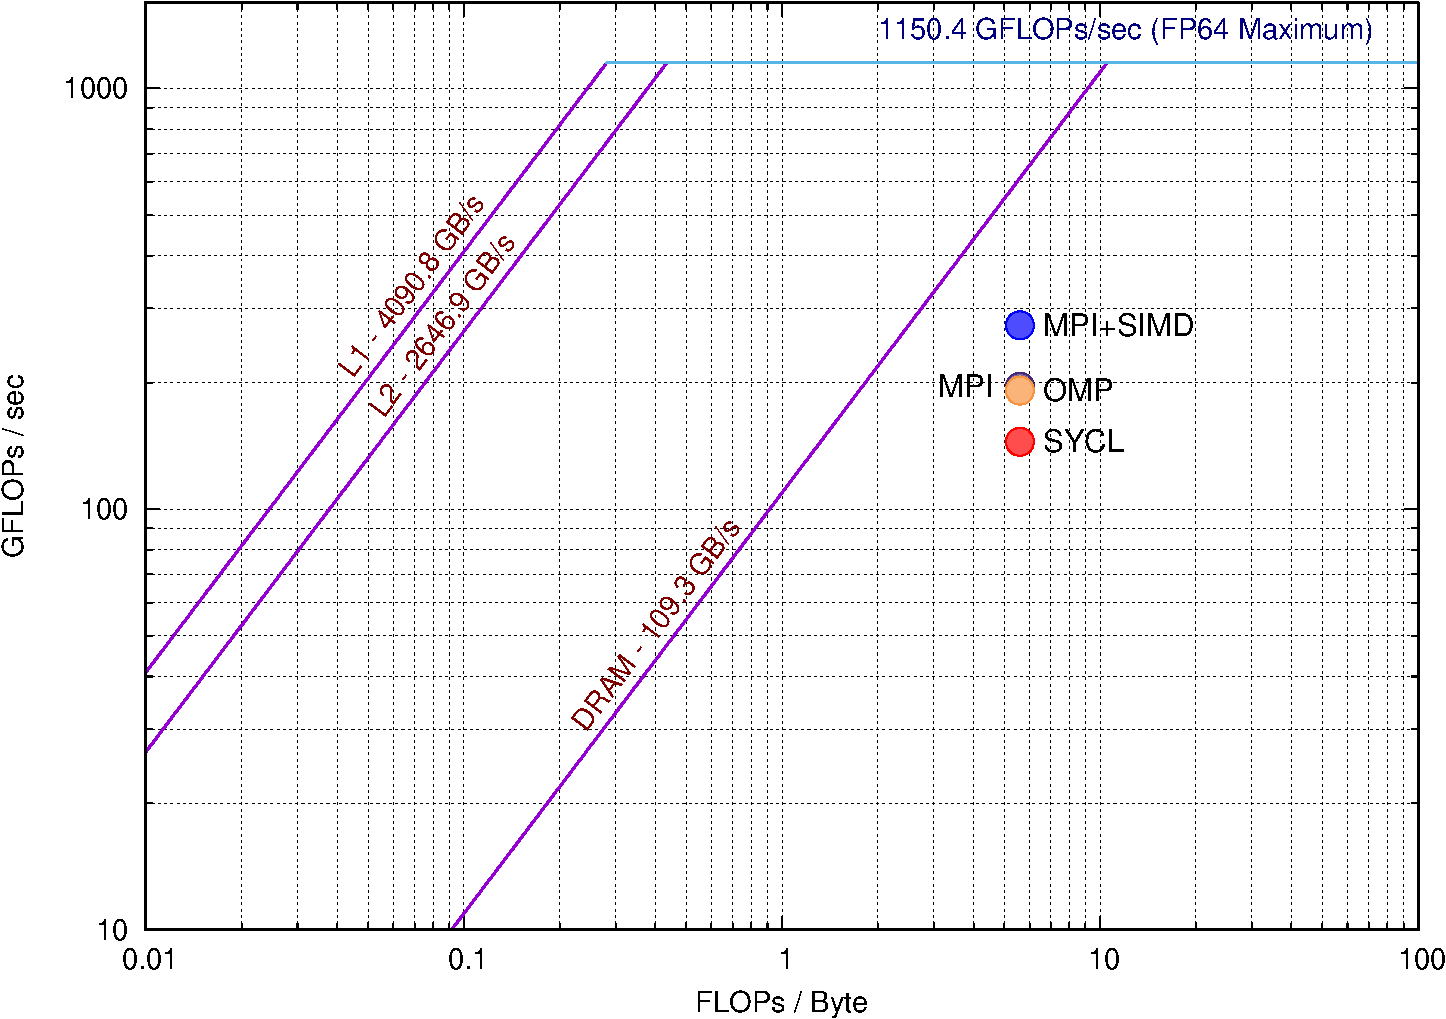
\includegraphics[width=6cm]{Rooflines/Roofline_platinum}  
% \caption{Intel Xeon (Platinum) - 48$\times$ MPI+SIMD, 48$\times$ MPI, 48$\times$ SMT 
% SYCL, 48$\times$ OpenMP}
% \label{graph/perf/platinum/roofline}
% \end{subfigure}
% \begin{subfigure}{.32\textwidth}\centering
% 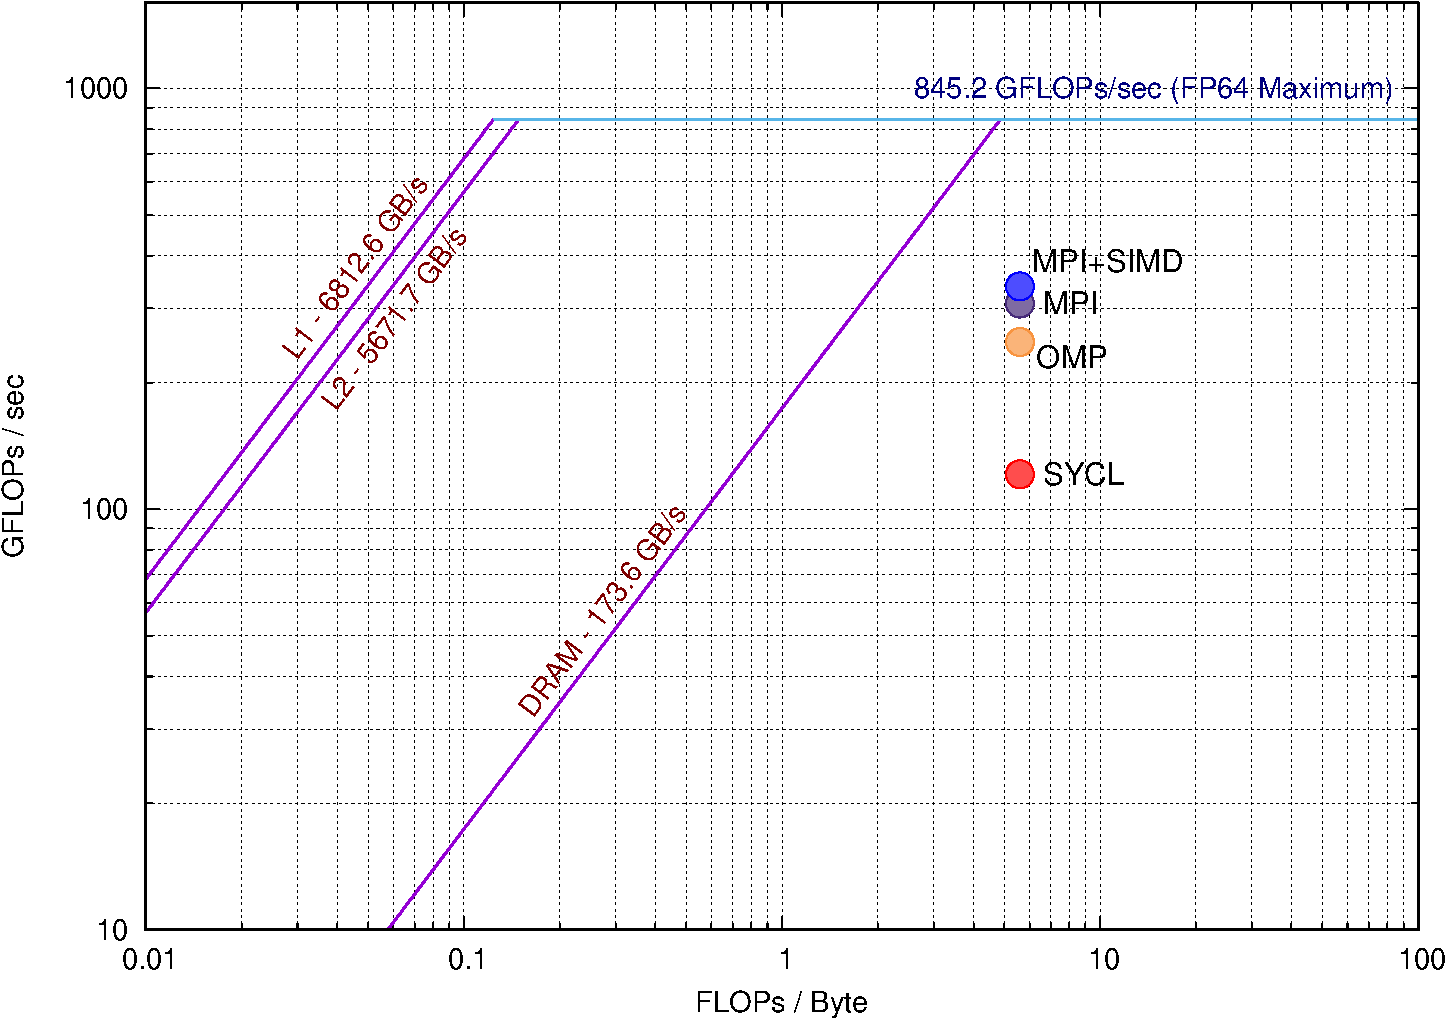
\includegraphics[width=6cm]{Rooflines/Roofline_graviton} 
% \caption{ARM Graviton - 64$\times$ MPI+SIMD, 64$\times$ MPI, 64$\times$ SMT 
% SYCL, 64$\times$ OpenMP}
% \label{graph/perf/isambard/roofline}
% \end{subfigure}
% \begin{subfigure}{.32\textwidth}
% 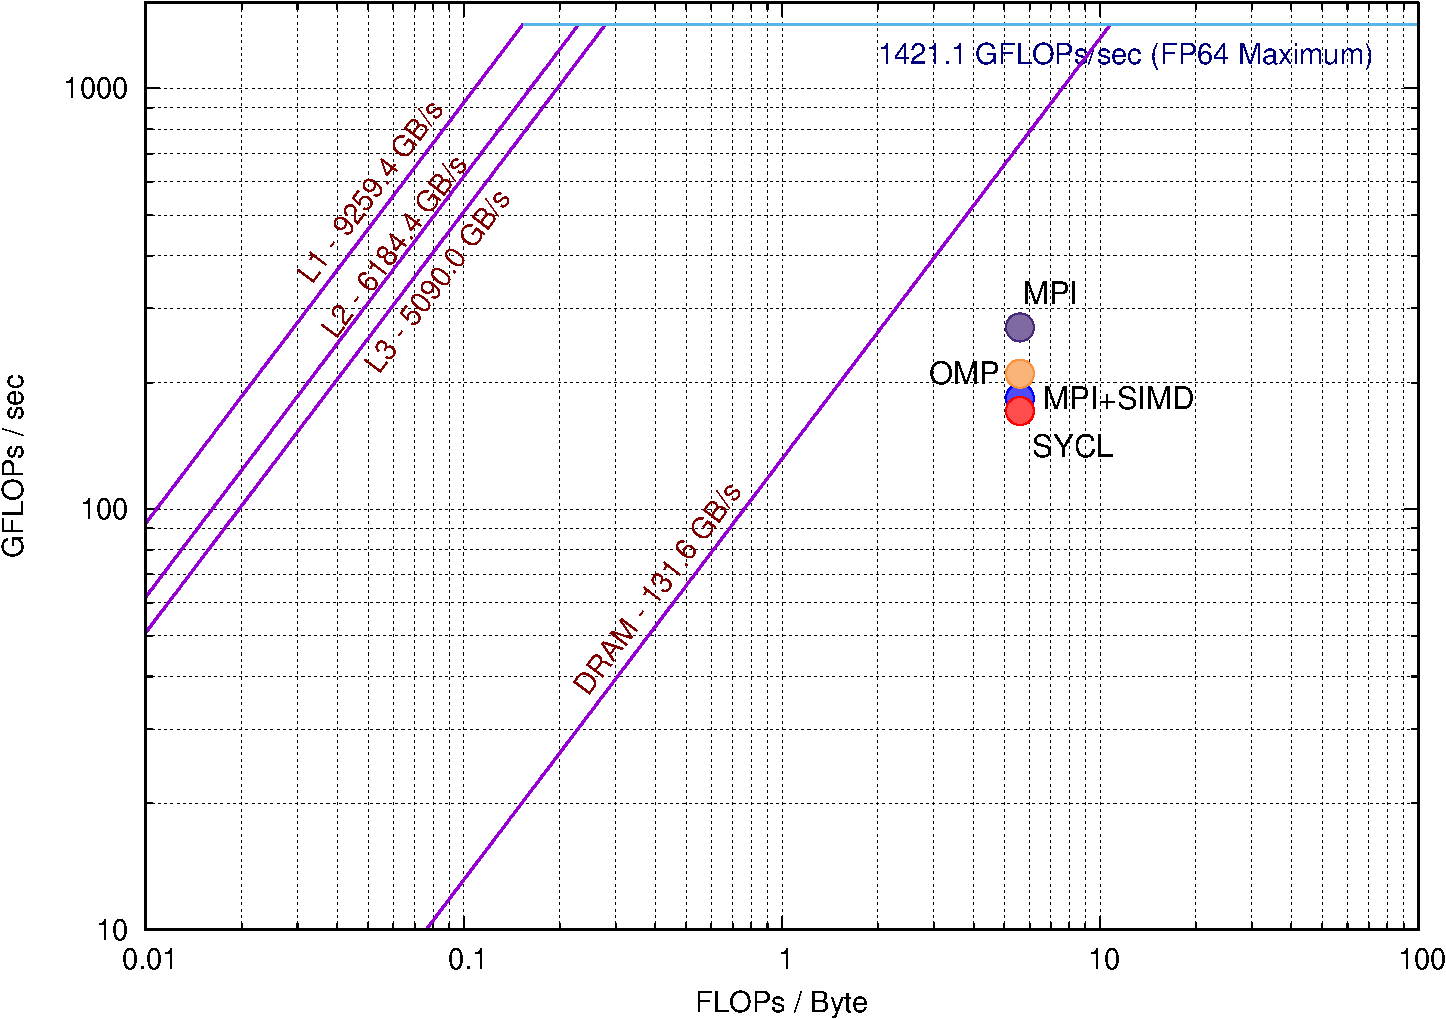
\includegraphics[width=6cm]{Rooflines/Roofline_amd} 
% \caption{AMD Epyc - 96$\times$ MPI+SIMD, 96$\times$ MPI, 96$\times$ SMT SYCL, 
% 48$\times$ OpenMP}
% \label{graph/perf/epyc/roofline}
% \end{subfigure}\vspace{-5pt}
% \caption{Roofline plots 1SKT CPU systems}
% \label{fig:fig}\vspace{-5pt}
% \end{figure*}\normalsize



\vspace{-10pt}
\section{Roofline Model Analysis}\label{sec/roof}
\vspace{-5pt}

\noindent To gather a further insight into the performance profile of the 
application, we picked the most time-consuming kernel 
(\texttt{compute\_flux\_edge}), responsible for over 50\% of total runtime to 
carry out a roofline model analysis. This kernel operates on edges, for each 
performing about 150 floating point instructions, reading 5 values from each 
node, 3 values from the edge, then indirectly incrementing 5 further values on 
each node. Due to the indirect accesses it is not a trivially vectorizable 
kernel, and it is highly sensitive to data reuse. For each platform we collected 
the relevant FLOPSs/Byte and GFLOPS/sec values onto the rooflines of each 
platform using the Berkeley Empirical Roofline Tool~\cite{lo2014roofline}.

\begin{table}[]\centering
\vspace{-15pt}\caption{Floating point instructions per edge with different 
compilers}
\renewcommand{\arraystretch}{1.2}
\label{tab:ops}
\begin{tabular}{@{}r|rr|rrr|r@{}}
\hline
&\multicolumn{2}{c|}{Scalar}  & \multicolumn{3}{c|}{SIMD}     &\ CUDA \\
&Intel\   &\ ARM/AMD\ \ &\ AVX 512 Intel\ \ &\ AVX  &\ ARM\ \ & \\\hline
FLOPs/edge\  \ & 150\   & 165\  \ & 216  & 165  & 164\ \  & 323\ \   \\\hline
FLOPs/byte\ \  & 2.52\  & 2.72\ \ & 3.63 & 2.77 & 2.72\ \ & 5.43\ \  \\\hline
\end{tabular}\vspace{-15pt}
\end{table}




\begin{figure*}[!h]\centering   \footnotesize 
\subfloat[Intel Cascade Lake
\label{graph/perf/platinum/roofline}] {
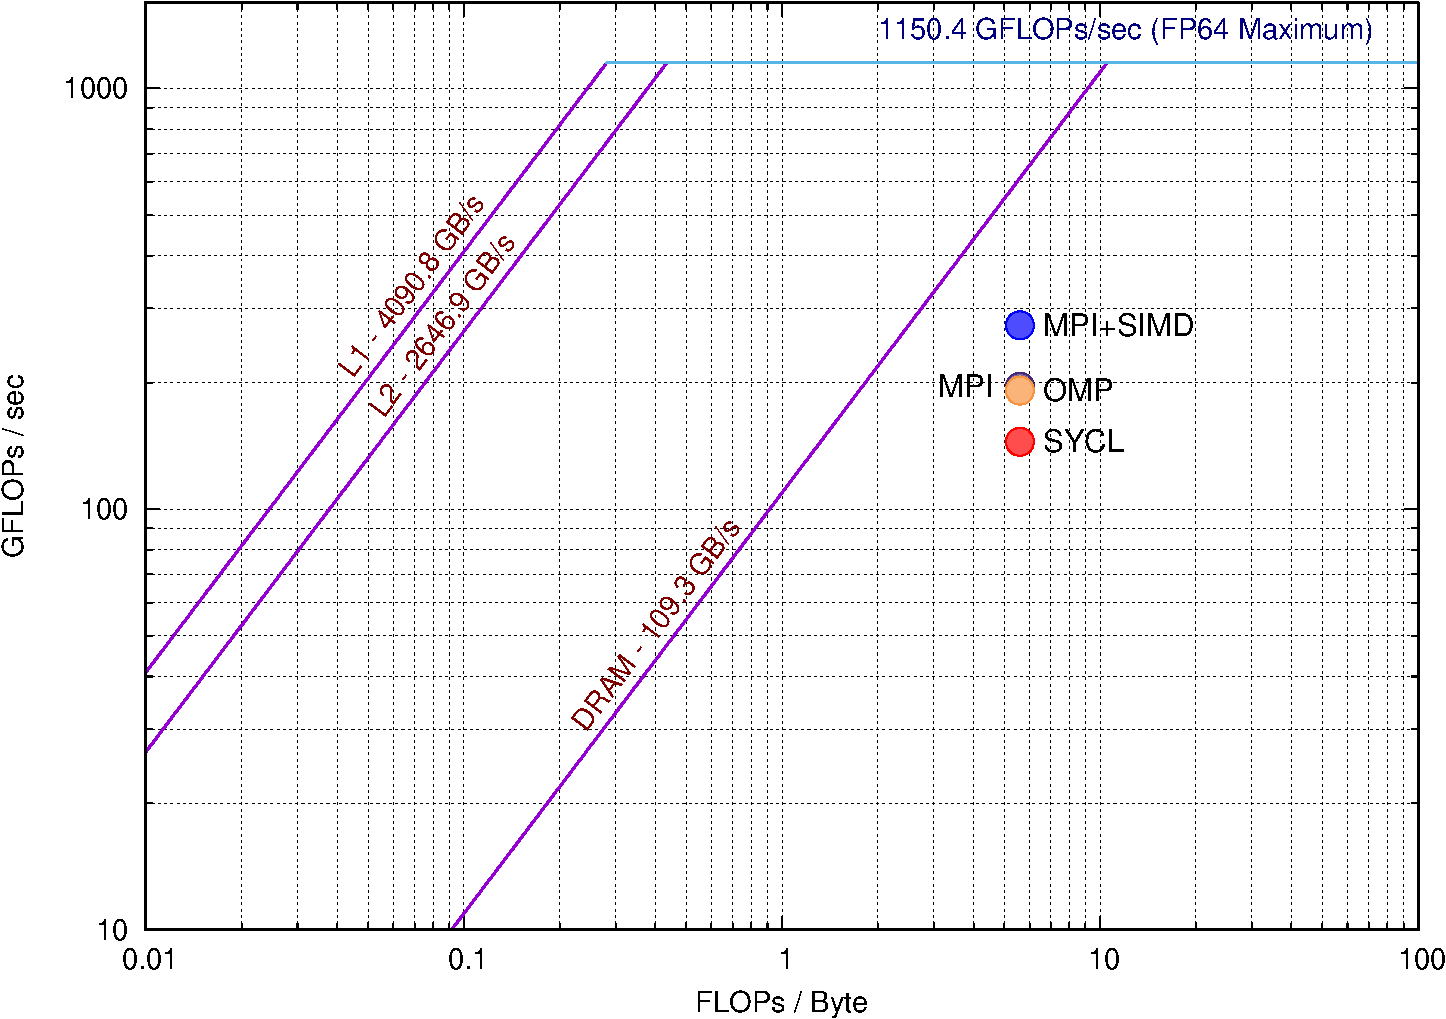
\includegraphics[width=8cm]{Rooflines/Roofline_platinum}  
}\\
\subfloat[ARM Graviton2
\label{graph/perf/isambard/roofline}] {
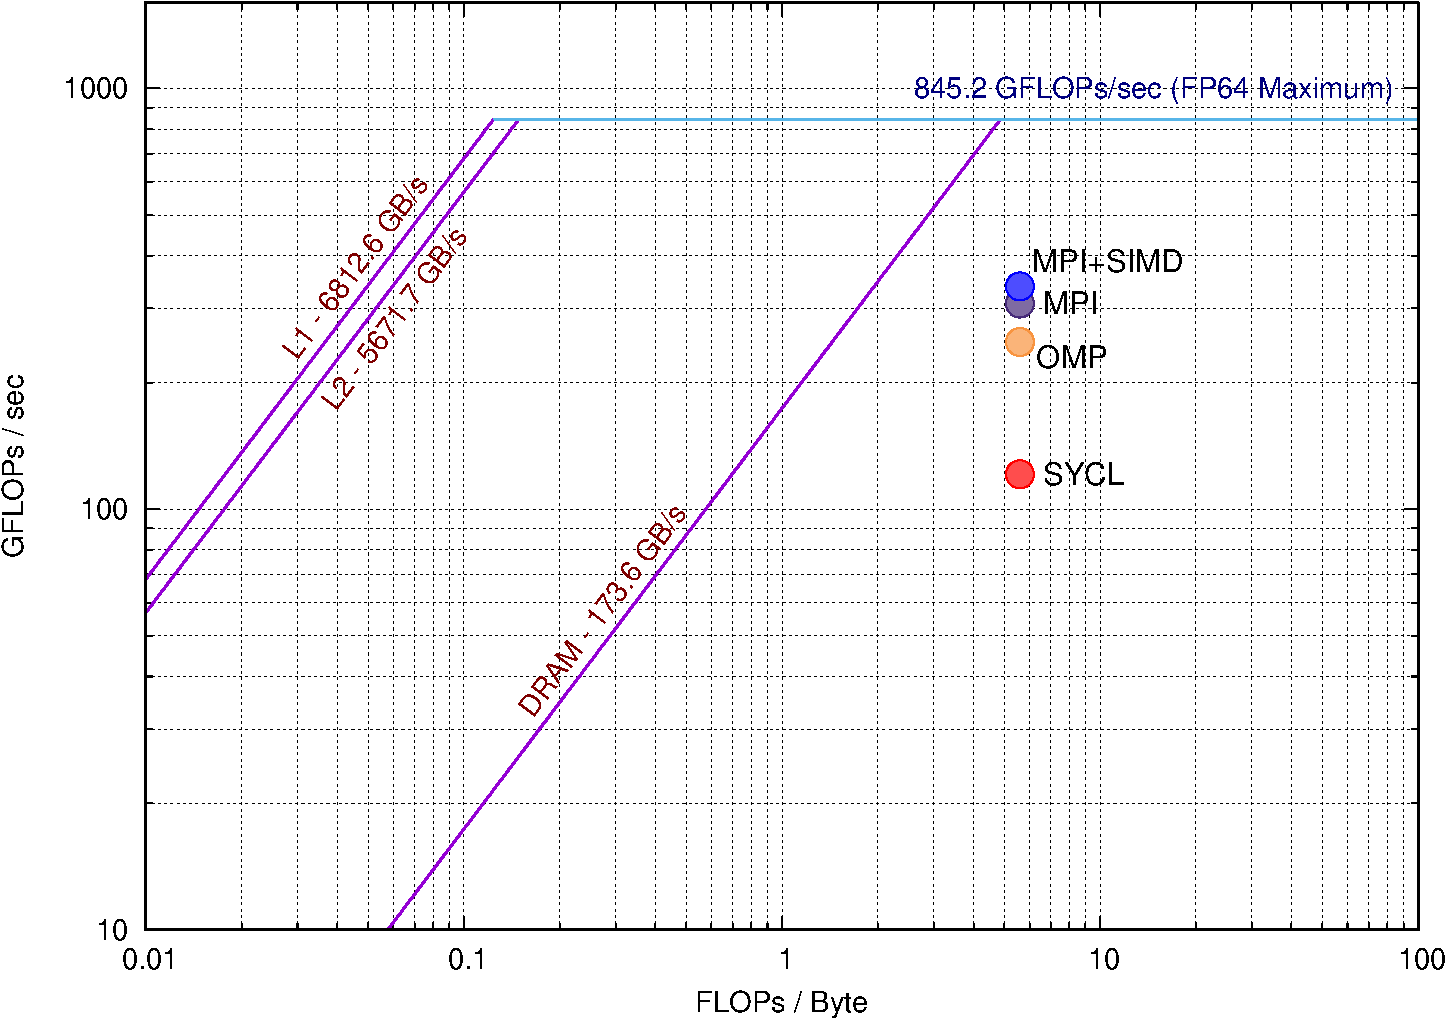
\includegraphics[width=8cm]{Rooflines/Roofline_graviton}  
}\\
\subfloat[AMD Epyc
\label{graph/perf/epyc/roofline}] {
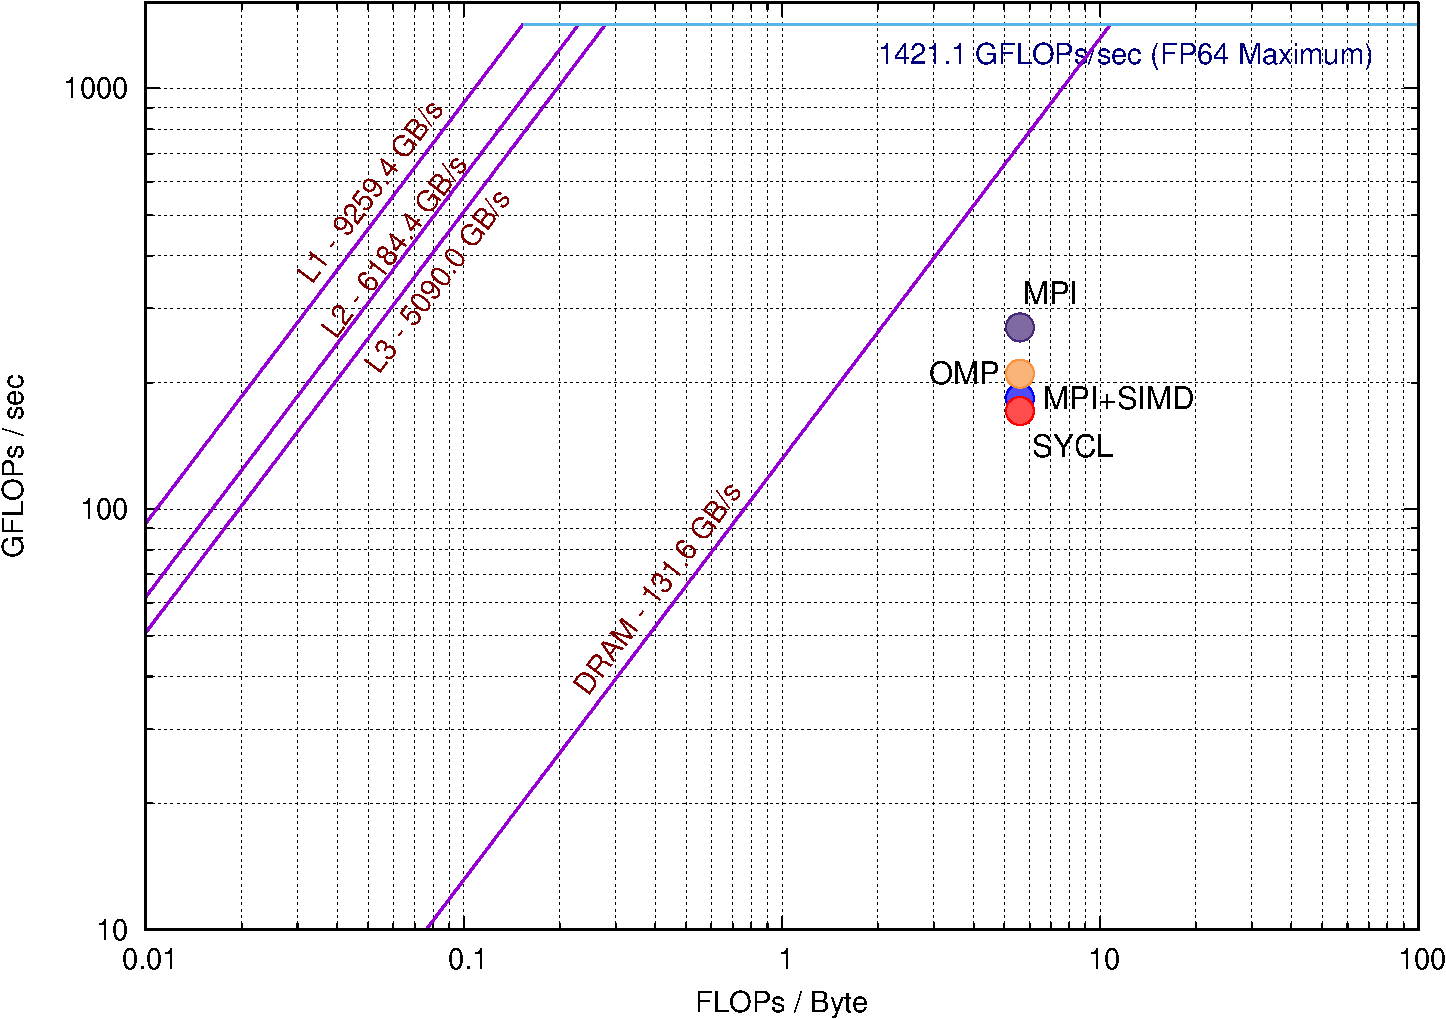
\includegraphics[width=8cm]{Rooflines/Roofline_amd}  
}\vspace{-2pt}
\caption{Roofline plots 1SKT CPU systems}
\label{fig:fig}\vspace{-50pt}
\end{figure*}\normalsize


\begin{figure*}[t]\centering    
\subfloat[NVIDIA V100] {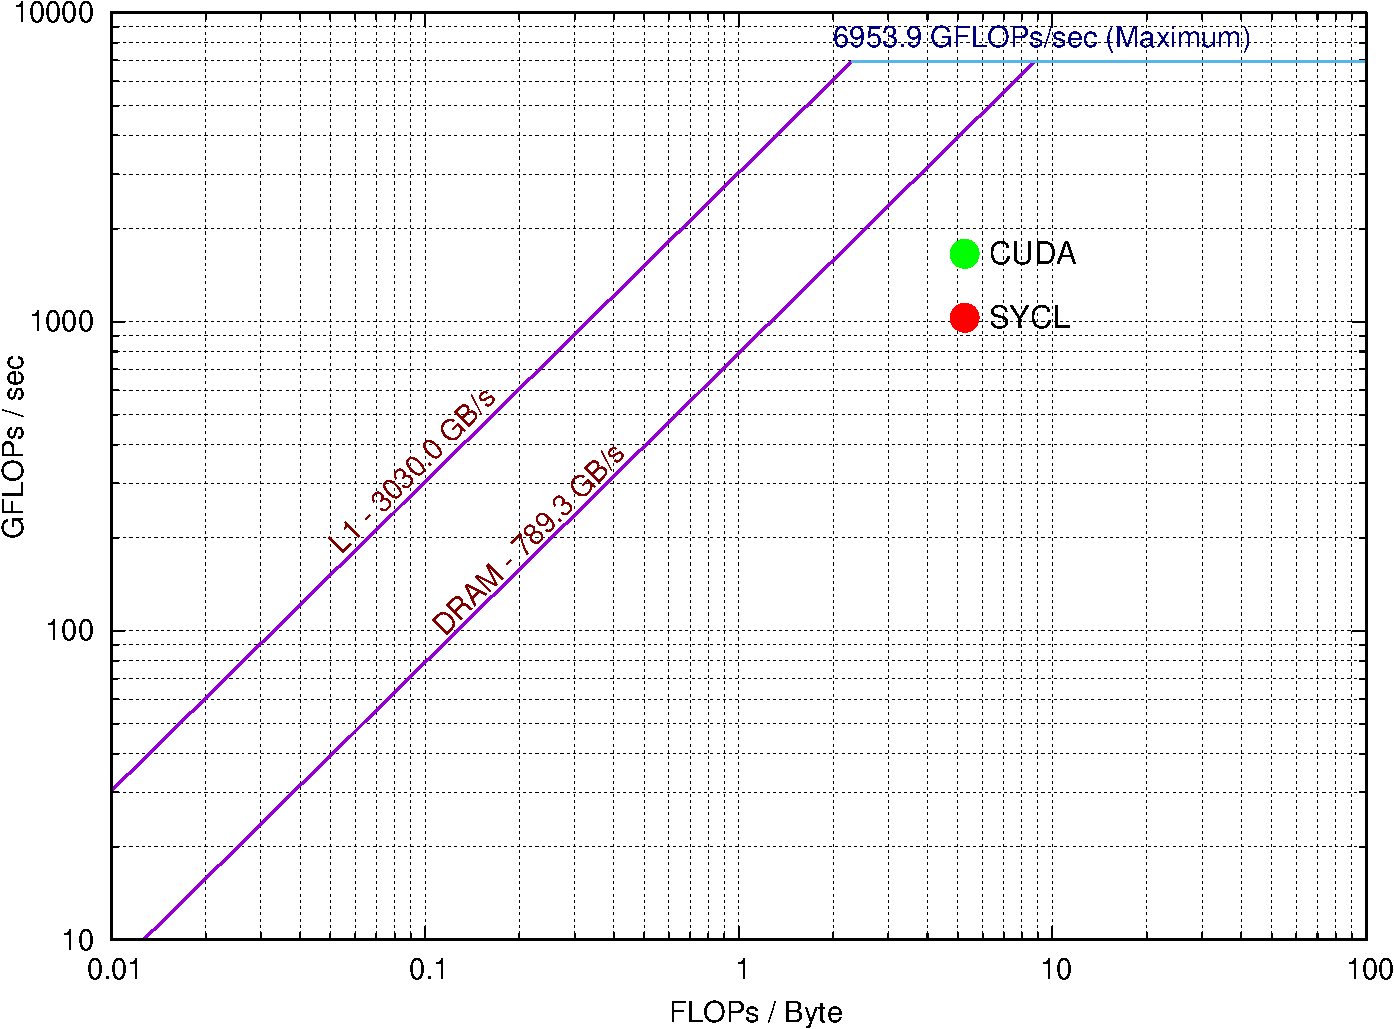
\includegraphics[width=8cm]{Rooflines/Roofline_V100}
\label{graph/perf/v100/roofline}}\\
\subfloat[NVIDIA A100\label{graph/perf/a100/roofline}] 
{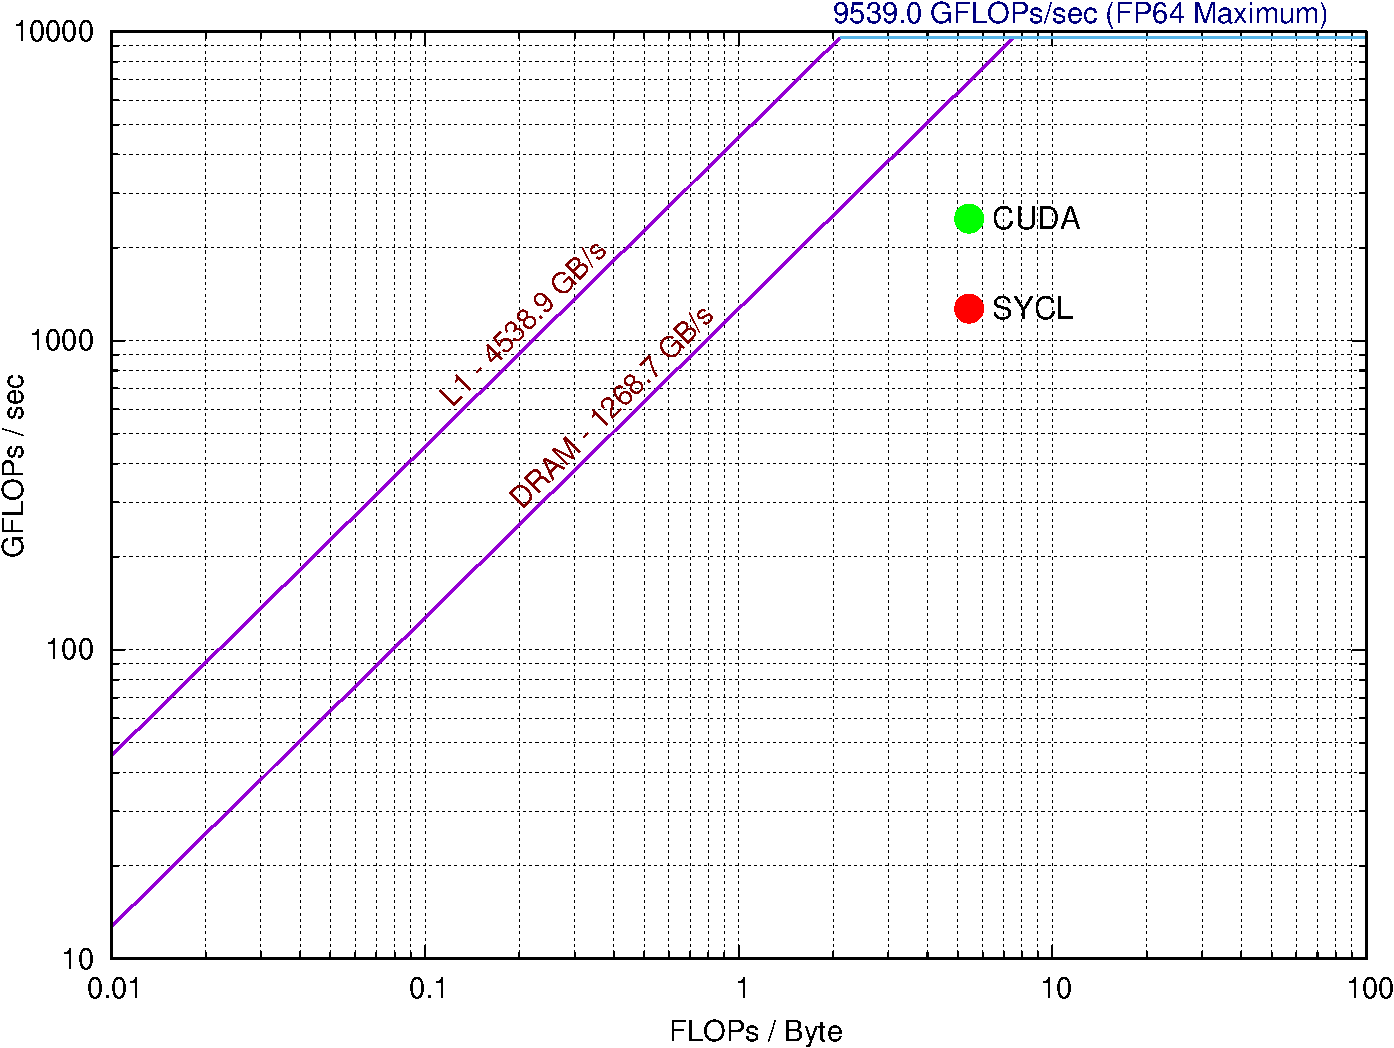
\includegraphics[width=8cm]{Rooflines/Roofline_A100}}
\vspace{-5pt}\caption{Roofline plots - NVIDIA GPUs}
\label{fig:roofline_nvidia_gpu}\vspace{-15pt}
\end{figure*}\normalsize

\begin{figure*}[t]\centering 
\subfloat[AMD Radeon VII\label{graph/perf/radeon/roofline}]
{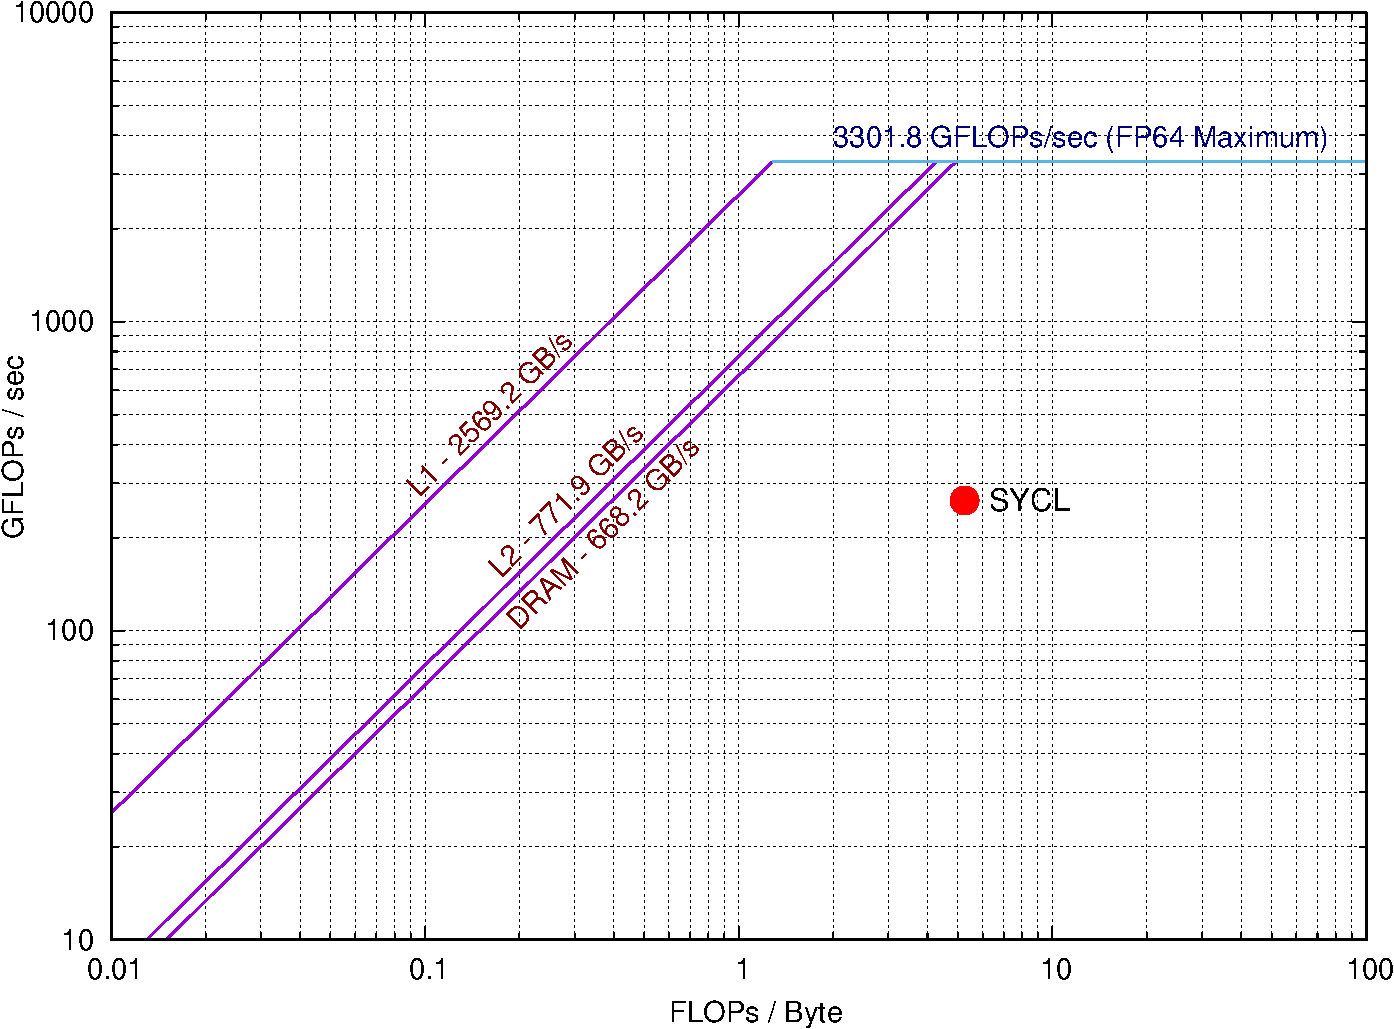
\includegraphics[width=8cm]{Rooflines/Roofline_RadionII}}\\
\subfloat[Intel Iris XE MAX (single 
precision)\label{graph/perf/xemax/roofline}] 
{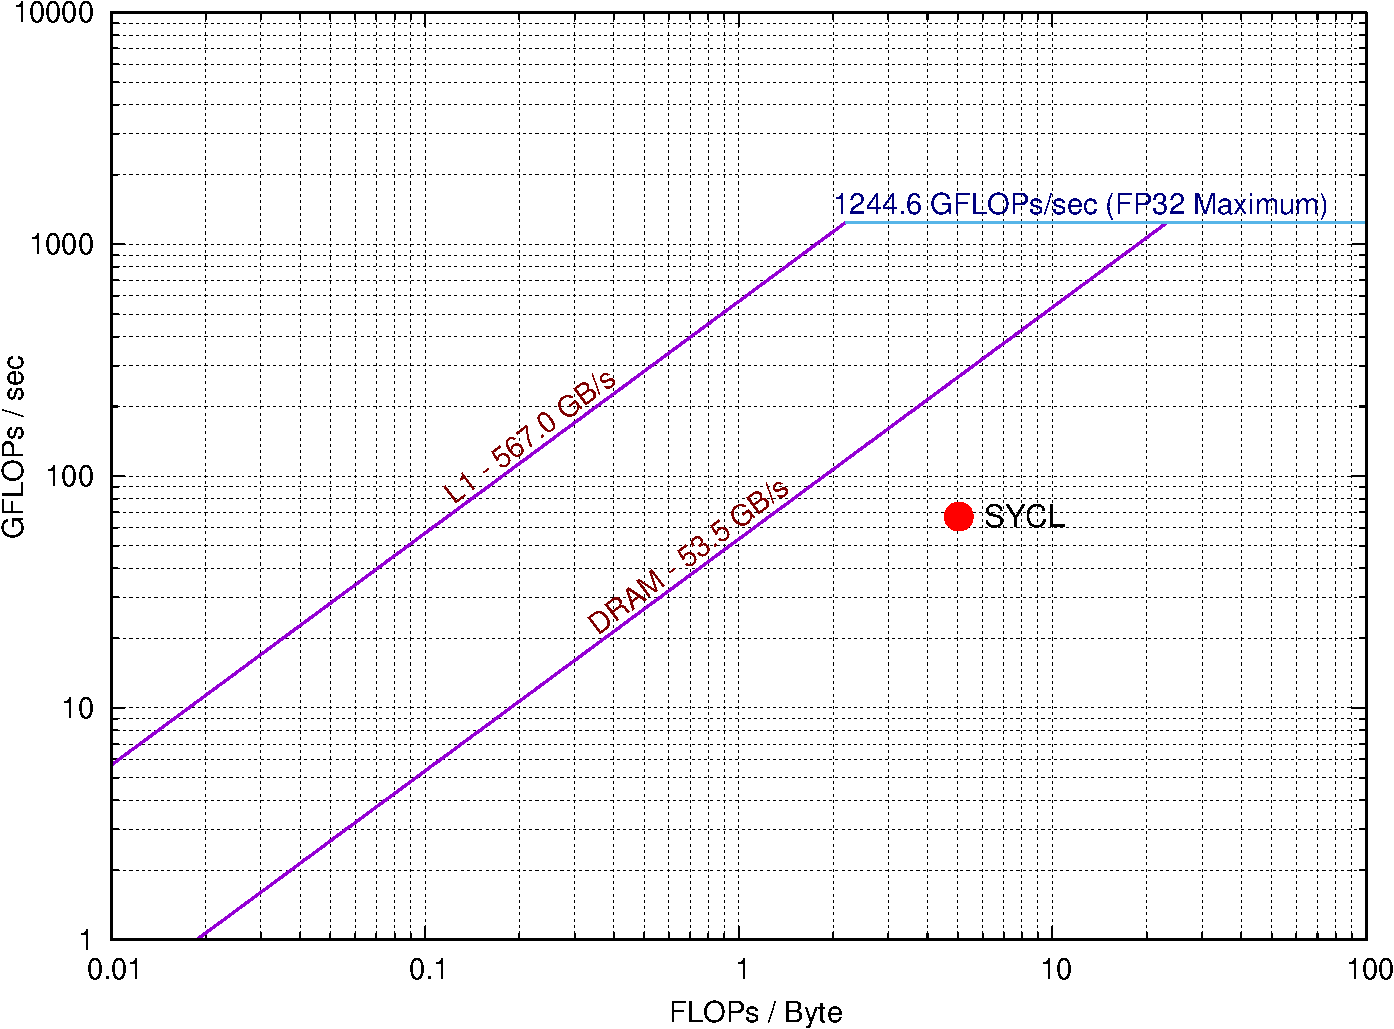
\includegraphics[width=8cm]{Rooflines/Roofline_IRIS}}
\vspace{-5pt}\caption{Roofline plots - Intel and AMD GPUs}
\label{fig:roofline_other_gpu}\vspace{-15pt}
\end{figure*}\normalsize

To calculate the operational intensity (FLOPs/byte) we inspected the assembly 
generated for the computation of each edge for different implementations. There 
are over 150 floating point operations per edge (varies slightly between 
compilers), and 13 of these are \texttt{sqrt} and \texttt{div} operations. It 
is important to note here that on CPUs there are separate assembly instructions 
for division and square root operations (though with much lower throughput than 
multiply or add), whereas on NVIDIA GPUs, these are mapped to a sequence of 
multiplications and additions. Furthermore, depending on the compiler and the 
kinds of vectors used (scalar, AVX or AVX512) we get different FLOP counts; for 
AVX precise divisions are used (single instruction), whereas with AVX512 
approximate reciprocals are used, followed by a number of additional multiply 
and add operations. Additionally, with SIMD and hierarchical execution schemes 
we stage increments in a local array, then apply them separately, adding a 
further 10 add instructions per edge. The number of floating point instructions 
per edge are reported in Table \ref{tab:ops}. For the amount of data moved, we 
did a calculation based on the number and size of data arrays accessed, assuming 
perfect data reuse, thereby intentionally omitting cache effects. The overall 
operational intensity is reported in Table \ref{tab:ops}.\\
\indent Figure~\ref{graph/perf/platinum/roofline} shows that on the Intel Xeon 
system, the 48 MPI+SIMD performance offers the best performance. The other 
parallel runs, which are plain 48 MPI, 1-socket SYCL, and 48 OpenMP show the 
same operational intensity, with the MPI and OpenMP versions being faster than 
the SYCL implementation. With Figure~\ref{graph/perf/isambard/roofline}, the 
picture with Graviton2 is similar to that of the Xeon system, except achieved 
performance of non-vectorized versions is higher, thanks to the higher 
achievable bandwidth and the shorter vector units. The gap between SYCL and 
other implementations is the largest on this platform, which is likely due to 
less optimized runtimes on ARM. Figure~\ref{graph/perf/epyc/roofline} shows the 
roofline for the AMD EPYC platform, here the SIMD variant does not improve 
performance. The gap between SYCL and other implementations is the narrowest 
thanks to the large bandwidth and the little impact from the lack of 
vectorization.\\
\indent The Nvidia GPU rooflines, seen in Figure~\ref{graph/perf/v100/roofline} 
for V100 and \ref{graph/perf/a100/roofline} for A100, show a similar picture, 
with both the SYCL and CUDA runs showing memory bound behavior (27\% and 18\% 
of peak respectively for SYCL). The Radeon VII roofline, shown in 
Figure~\ref{graph/perf/radeon/roofline}, achieves a lower 15.6\% fraction of 
peak, because it uses a hierachical execution scheme that requires increased 
coordination between threads. Finally, the Iris XE MAX, running in single 
precision is clearly much more bound by memory bandwidth, and also uses the 
hierarchical execution scheme, yet achieves 24.8\% of peak.



%, with the arithmetic 
%intensity being decreased due to the use of 512-bit wide vector instructions. 

% \begin{figure*}[t]\centering   \footnotesize 
% \begin{subfigure}{.32\textwidth}
% 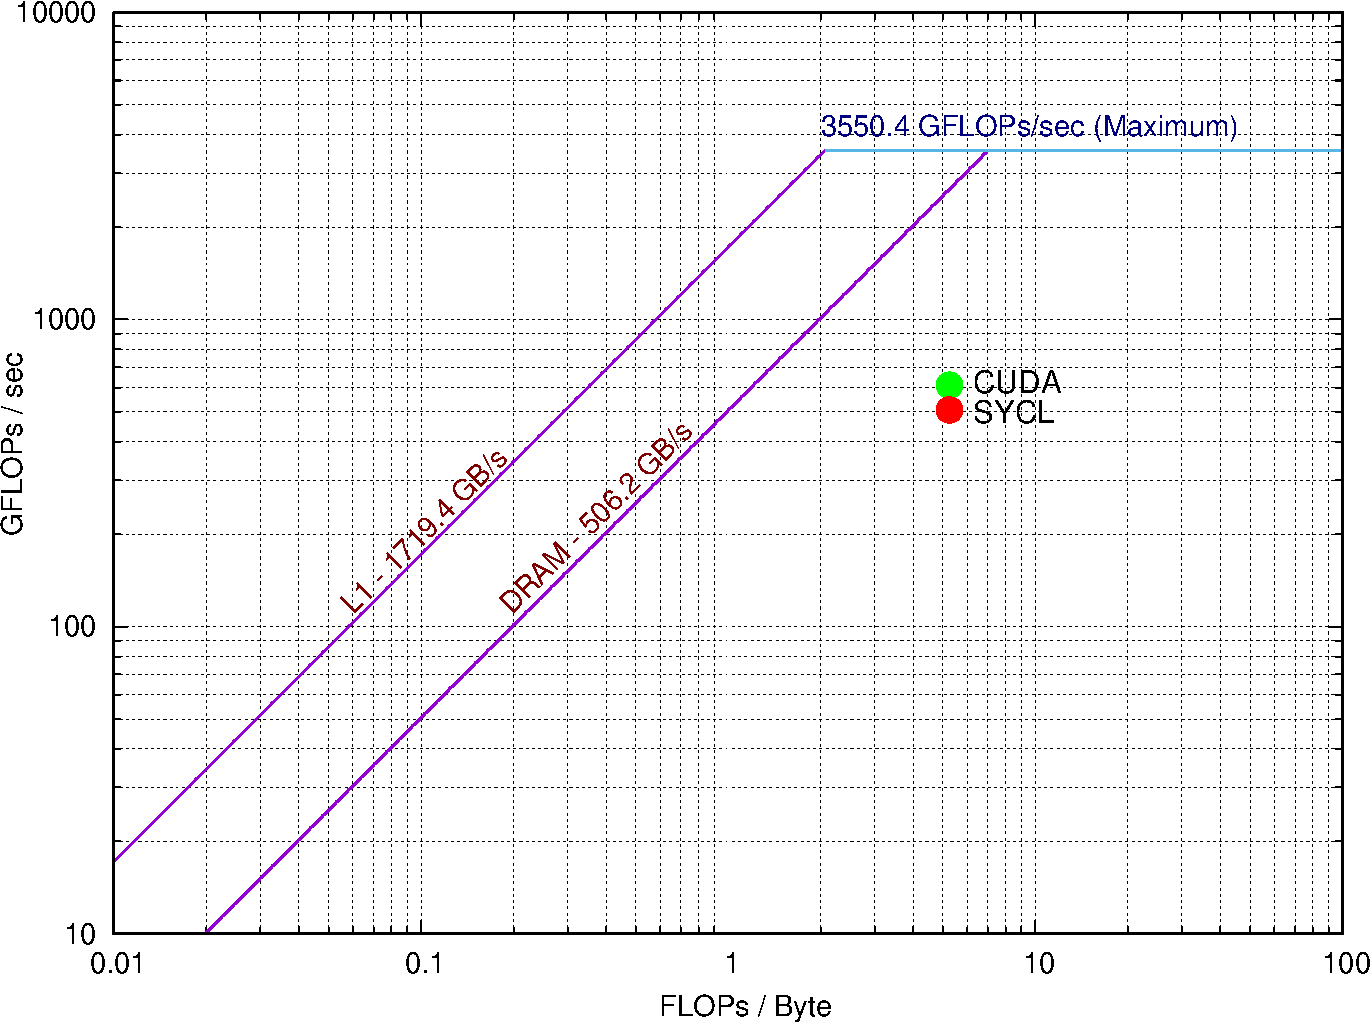
\includegraphics[width=6cm]{Rooflines/Roofline_P100}  
% \caption{P100, CUDA and SYCL}
% \label{graph/perf/p100/roofline}
% \end{subfigure}
% \begin{subfigure}{.32\textwidth}
% 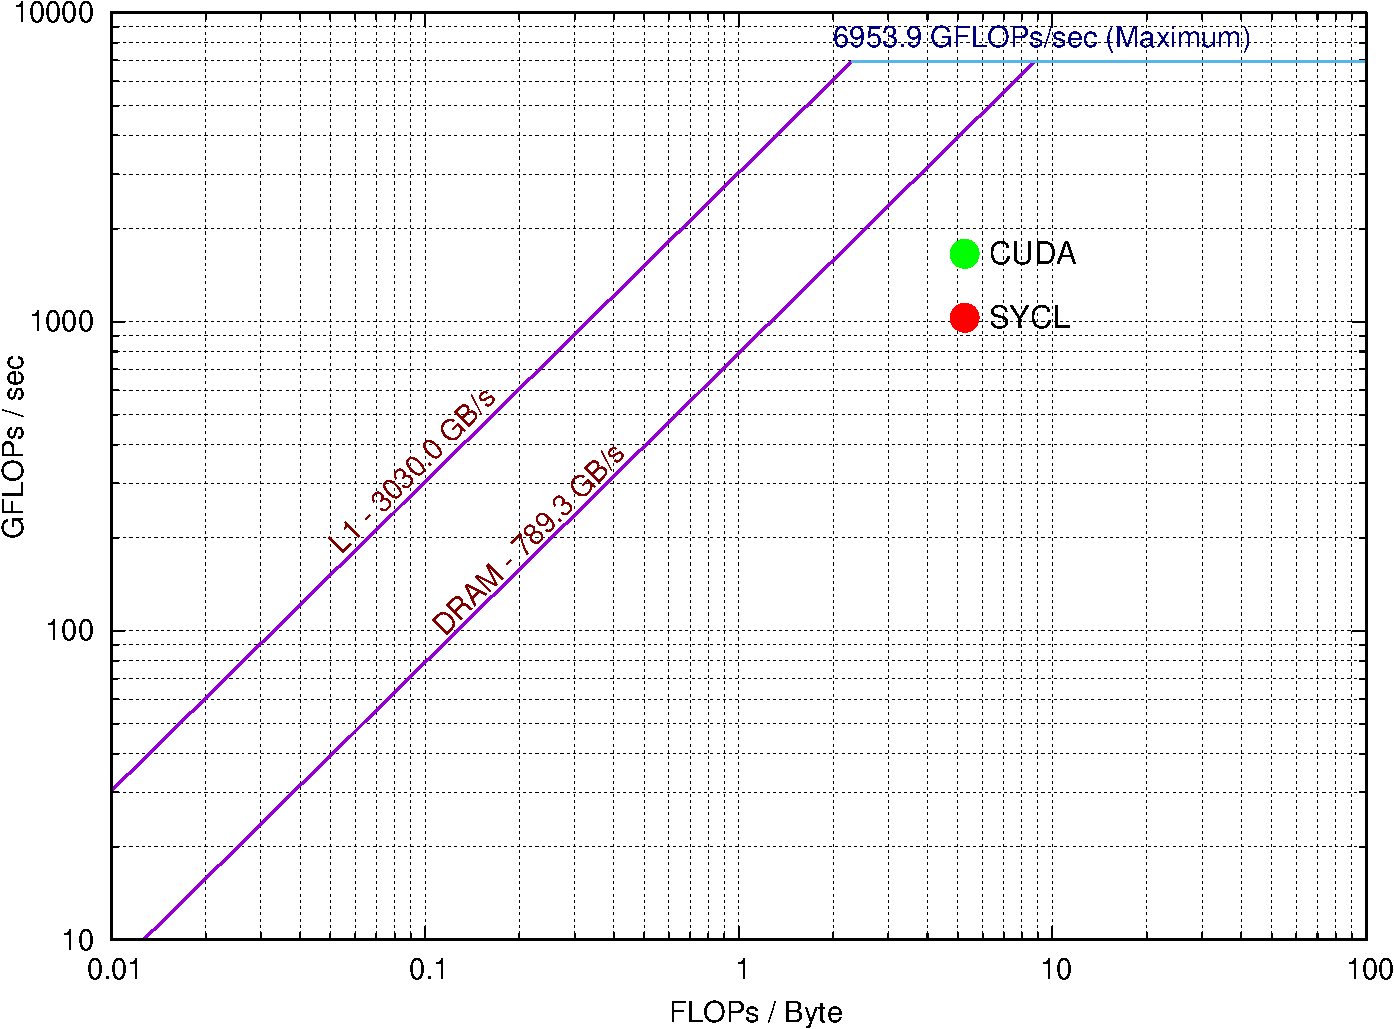
\includegraphics[width=6cm]{Rooflines/Roofline_V100} 
% \caption{V100, CUDA and SYCL}
% \label{graph/perf/v100/roofline}
% \end{subfigure}
% \begin{subfigure}{.32\textwidth}
% 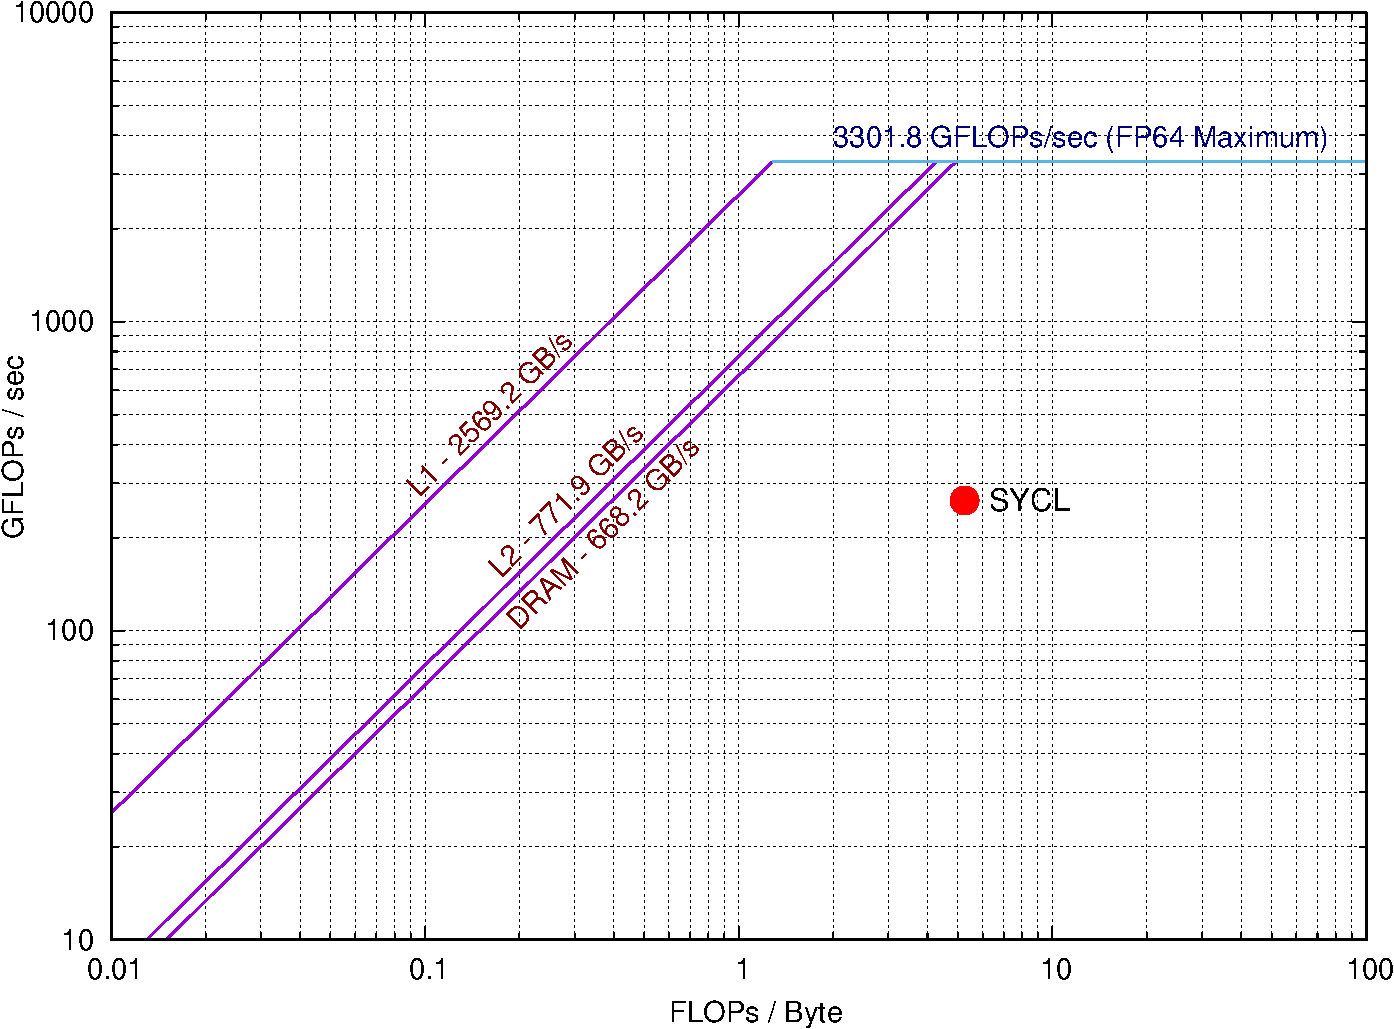
\includegraphics[width=6cm]{Rooflines/Roofline_RadionII} 
% \caption{Radeon VII, SYCL}
% \label{graph/perf/radeon/roofline}
% \end{subfigure}
% \caption{Roofline plots for NVIDIA P100, V100 and AMD Radeon VII}
% \label{fig:fig}\vspace{-6pt}
% \end{figure*}\normalsize


%further confirms our observation. This 
%would explain why the Radeon VII is able to attain such impressive performance. 
%Along side the NVIDIA GPUs, the Radeon VII has low floating point double 
%precision performance, with only 3.5 TFLOPS FP64\cite{RadeonVIIspec} compared 
%to the NVIDIA's V100 with 7 TFLOPS FP64~\cite{V100TDP}. If the 
%\texttt{compute\_flux\_edge\_kernel} loop was compute bound, then the Radeon VII 
%would exhibit significantly slower performance than the Nvidia GPU. Instead, the 
%Radeon VII SYCL runtime is 58\% faster than the V100 using CUDA, which may 
%in-part be explained by the higher memory bandwidth (1024 GB/s vs. 900 GB/s). 
% Overall, the SYCL versions show similar roofline behavior as the other specific 
% parallel programming models such as MPI, CUDA and OpenMP.



% \begin{figure}[!t]\hspace{-0pt}
% 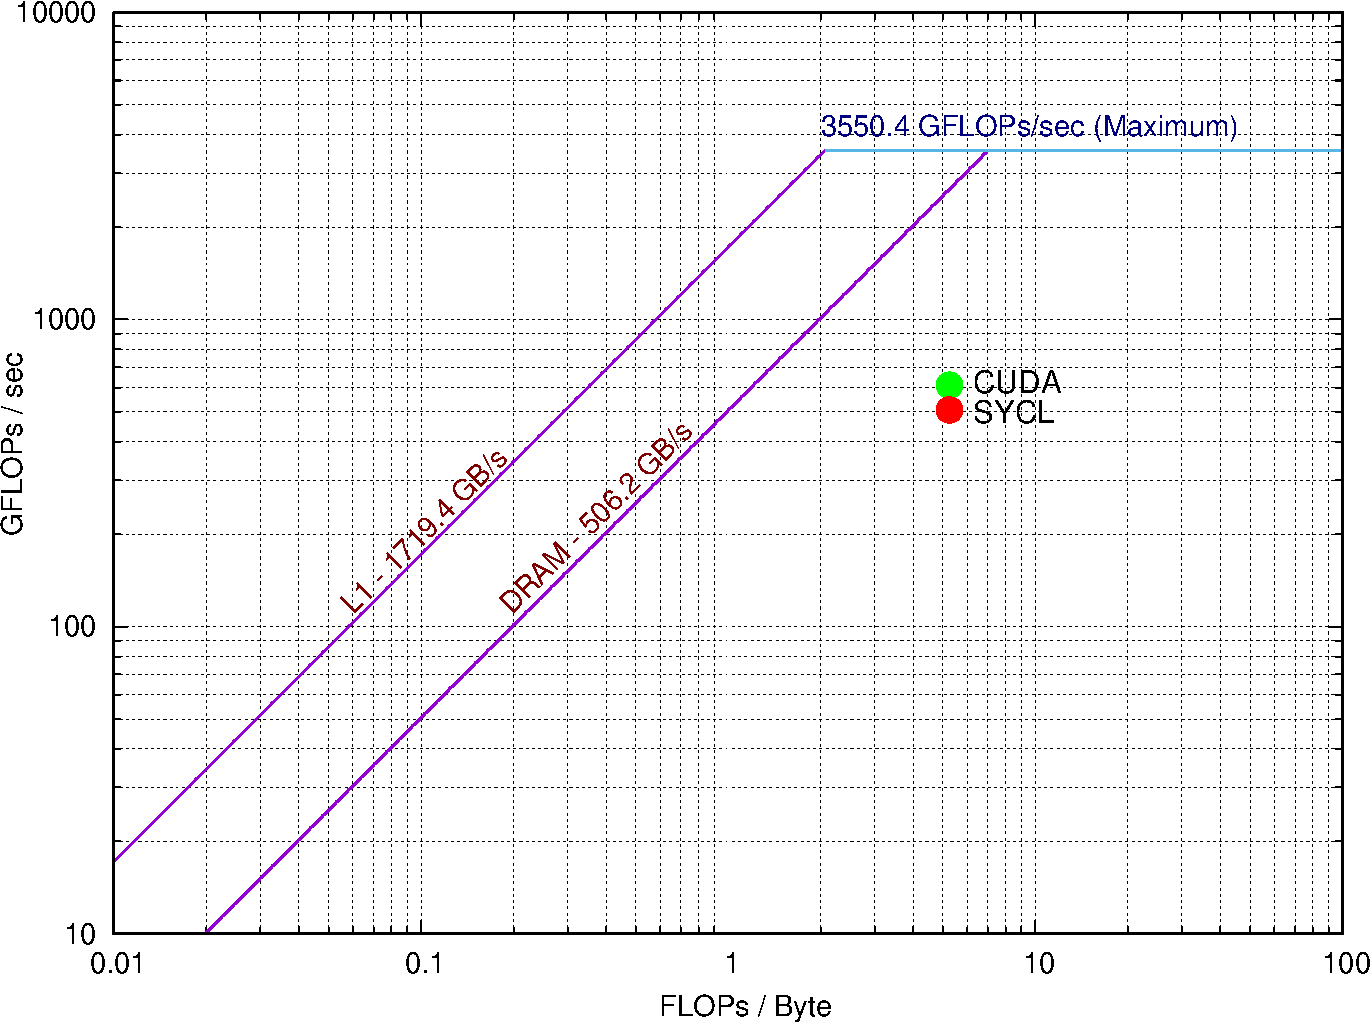
\includegraphics[height=5cm]{Rooflines/Roofline_P100} \vspace{-3pt}
% \caption{Roofline plot of the Nvidia P100, showing the CUDA and SYCL performance}
% \label{graph/perf/p100/roofline}\vspace{-10pt}
% \end{figure}

% \begin{figure}[!t]\hspace{-0pt}
% 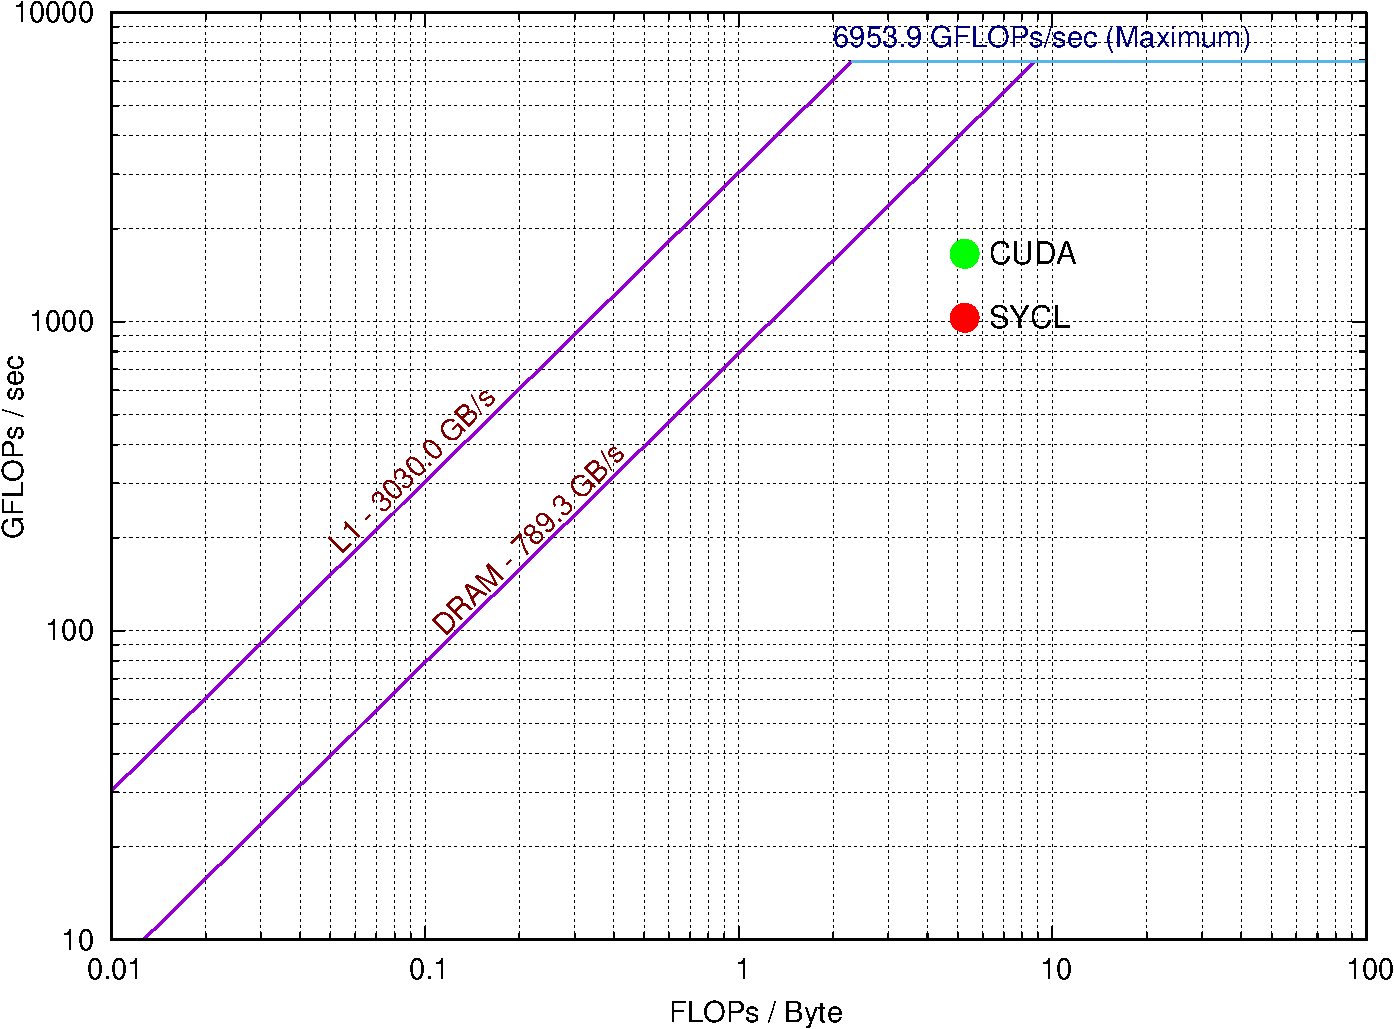
\includegraphics[height=5cm]{Rooflines/Roofline_V100} \vspace{-3pt}
% \caption{Roofline plot of the Nvidia V100, showing the CUDA and SYCL 
% performance}
% \label{graph/perf/v100/roofline}\vspace{-10pt}
% \end{figure}

% \begin{figure}[!t]\hspace{-0pt}
% 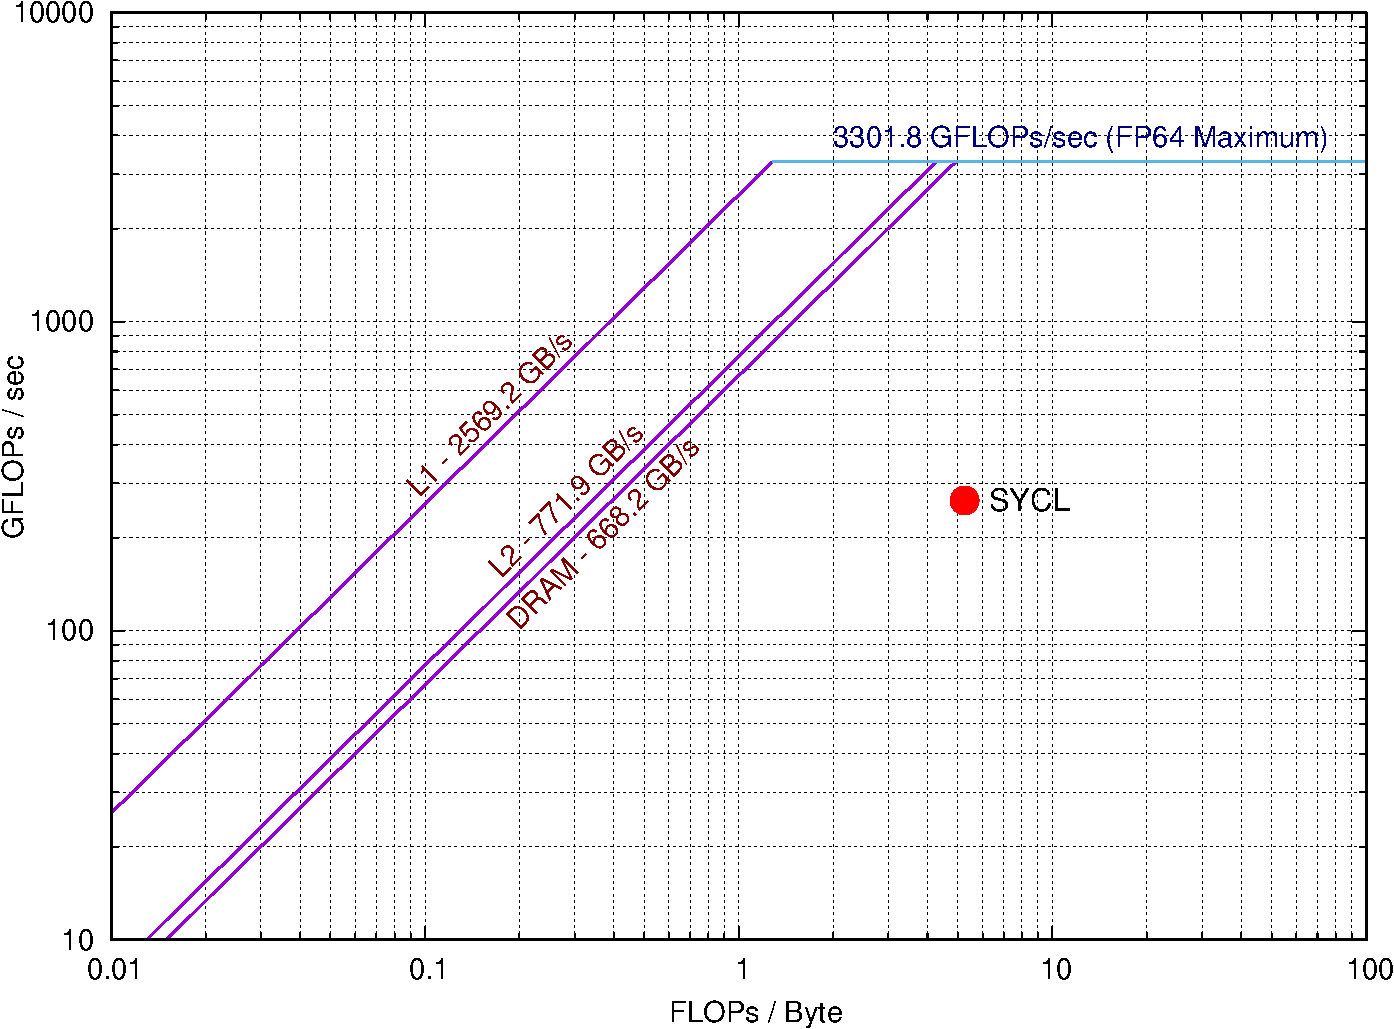
\includegraphics[height=5cm]{Rooflines/Roofline_RadionII} 
% \vspace{-3pt}
% \caption{Roofline plot of the AMD Radeon VII, showing the SYCL performance}
% \label{graph/perf/radeon/roofline}\vspace{-10pt}
% \end{figure}


% However, the need to ``writing'' two different parallelizations (in this case 
% coloring for CPUs and atomics for GPUs) are still there with OneAPI

\vspace{-5pt}
\section{Conclusion}\label{sec/conclusions}
\vspace{-5pt}
% Decent Performance across the board on CPUs and GPUs

\noindent The results shown indicate that the SYCL API brings comparable performance 
overall for both CPUs and GPUs from different vendors in this application. The 
SYCL ecosystem is rapidly closing the performance gap with other parallel 
programming models. This is an essential quality of any new parallel API, so the 
fact that SYCL already achieves this shows that it is a good foundation for 
Intel's OneAPI software suite. In addition, as the standard is further 
developed, performance parity with other models is expected as software and 
hardware vendors optimise. \\
\indent However, as we have shown, there is still the need to write different 
parallelizations within the code to achieve the best runtimes. In the case 
of this unstructured mesh application, that included writing a coloring 
parallelization for CPUs and Radeon GPUs, and an atomics version for 
NVIDIA GPUs. Thus, the idea of SYCL abstracting away device specific code may 
not be entirely representative of real world use cases. This is especially true 
for irregular classes of applications, such as unstructured-mesh as opposed to 
the more commonly explored regular applications.\\
\indent If this disparity continues, then it could lead to SYCL being seen as 
yet another industry standard, being grouped together with existing compute 
frameworks which offer similar levels of performance portability. For example, 
OpenMP 4.0 is a far more mature standard which can also be written for all 
devices that SYCL currently supports, not to mention code-bases that do not use 
modern C++ (e.g. Fortran), which then cannot use SYCL. The DSL-based code 
generator used in this work, OP2, has been able to keep up with such changes by 
adding another code generator which can adhere to new standards. However, for 
applications which are not based on frameworks and require a rewrite, developers 
could be hesitant to adopt SYCL for these reasons. 

% This could lead to Yet Another Industry ``Standard''? (YAIS)
% OP2 has been able to keep up with this YAIS issue by simply adding another 
% code-generator (YAIS-AAC)

% It is interesting to see the need for two contrasting parallelization strategies 
% to get best performance on different platforms. This poses the question whether 
% SYCL and in-turn OneAPI do indeed provide a unifying API that truly enables 
% performance portability.

% State that: it is interesting to see the need for two contrasting 
% parallelization strategies to get best performance on different platforms. 
% This puts poses the question whether SYCL and OneAPI in return do indeed 
% provide a unifying API that truly enable performance portability.  

% use section* for acknowledgment
\section*{Acknowledgment}
% \noindent This research is supported by Rolls-Royce plc and by the UK 
% Engineering and Physical Sciences Research Council (EPSRC): (EP/S005072/1 - 
% Strategic Partnership in Computational Science for Advanced Simulation and 
% Modelling of Engineering Systems - ASiMoV). Gihan Mudalige was supported by the 
% Royal Society Industry Fellowship Scheme(INF/R1/1800 12). The authors would 
% like to thank the GW4 Alliance and the University of Bristol for giving us 
% access to the Isambard system as well as the Radeon VII node in their HPC Zoo.
% Istv\'an Reguly was supported by National Research, Development and  Innovation 
% Fund of Hungary, project PD 124905, financed under the PD\_17 funding scheme.

\bibliographystyle{splncs04}
\bibliography{op2mgcfd.bib}


%\section*{Appendix - Reproducibility}

% See : 
% https://warwick.ac.uk/fac/sci/dcs/people/gihan_mudalige/heterogeneous-cpu-gpu_ca
% meraready.pdf

% MG-CFD code repo and branch URLs - including installation 
% OP2 code repo and branch URLs - including installation 
% Results data-set Excel sheet (Web URL)
% Raw runtime results tar ball (including Intel Advisor results)






\end{document}


